\documentclass[twoside]{book}

% Packages required by doxygen
\usepackage{fixltx2e}
\usepackage{calc}
\usepackage{doxygen}
\usepackage[export]{adjustbox} % also loads graphicx
\usepackage{graphicx}
\usepackage[utf8]{inputenc}
\usepackage{makeidx}
\usepackage{multicol}
\usepackage{multirow}
\PassOptionsToPackage{warn}{textcomp}
\usepackage{textcomp}
\usepackage[nointegrals]{wasysym}
\usepackage[table]{xcolor}

% Font selection
\usepackage[T1]{fontenc}
\usepackage[scaled=.90]{helvet}
\usepackage{courier}
\usepackage{amssymb}
\usepackage{sectsty}
\renewcommand{\familydefault}{\sfdefault}
\allsectionsfont{%
  \fontseries{bc}\selectfont%
  \color{darkgray}%
}
\renewcommand{\DoxyLabelFont}{%
  \fontseries{bc}\selectfont%
  \color{darkgray}%
}
\newcommand{\+}{\discretionary{\mbox{\scriptsize$\hookleftarrow$}}{}{}}

% Page & text layout
\usepackage{geometry}
\geometry{%
  a4paper,%
  top=2.5cm,%
  bottom=2.5cm,%
  left=2.5cm,%
  right=2.5cm%
}
\tolerance=750
\hfuzz=15pt
\hbadness=750
\setlength{\emergencystretch}{15pt}
\setlength{\parindent}{0cm}
\setlength{\parskip}{3ex plus 2ex minus 2ex}
\makeatletter
\renewcommand{\paragraph}{%
  \@startsection{paragraph}{4}{0ex}{-1.0ex}{1.0ex}{%
    \normalfont\normalsize\bfseries\SS@parafont%
  }%
}
\renewcommand{\subparagraph}{%
  \@startsection{subparagraph}{5}{0ex}{-1.0ex}{1.0ex}{%
    \normalfont\normalsize\bfseries\SS@subparafont%
  }%
}
\makeatother

% Headers & footers
\usepackage{fancyhdr}
\pagestyle{fancyplain}
\fancyhead[LE]{\fancyplain{}{\bfseries\thepage}}
\fancyhead[CE]{\fancyplain{}{}}
\fancyhead[RE]{\fancyplain{}{\bfseries\leftmark}}
\fancyhead[LO]{\fancyplain{}{\bfseries\rightmark}}
\fancyhead[CO]{\fancyplain{}{}}
\fancyhead[RO]{\fancyplain{}{\bfseries\thepage}}
\fancyfoot[LE]{\fancyplain{}{}}
\fancyfoot[CE]{\fancyplain{}{}}
\fancyfoot[RE]{\fancyplain{}{\bfseries\scriptsize Generated by Doxygen }}
\fancyfoot[LO]{\fancyplain{}{\bfseries\scriptsize Generated by Doxygen }}
\fancyfoot[CO]{\fancyplain{}{}}
\fancyfoot[RO]{\fancyplain{}{}}
\renewcommand{\footrulewidth}{0.4pt}
\renewcommand{\chaptermark}[1]{%
  \markboth{#1}{}%
}
\renewcommand{\sectionmark}[1]{%
  \markright{\thesection\ #1}%
}

% Indices & bibliography
\usepackage{natbib}
\usepackage[titles]{tocloft}
\setcounter{tocdepth}{3}
\setcounter{secnumdepth}{5}
\makeindex

% Hyperlinks (required, but should be loaded last)
\usepackage{ifpdf}
\ifpdf
  \usepackage[pdftex,pagebackref=true]{hyperref}
\else
  \usepackage[ps2pdf,pagebackref=true]{hyperref}
\fi
\hypersetup{%
  colorlinks=true,%
  linkcolor=blue,%
  citecolor=blue,%
  unicode%
}

% Custom commands
\newcommand{\clearemptydoublepage}{%
  \newpage{\pagestyle{empty}\cleardoublepage}%
}

\usepackage{caption}
\captionsetup{labelsep=space,justification=centering,font={bf},singlelinecheck=off,skip=4pt,position=top}

%===== C O N T E N T S =====

\begin{document}

% Titlepage & ToC
\hypersetup{pageanchor=false,
             bookmarksnumbered=true,
             pdfencoding=unicode
            }
\pagenumbering{alph}
\begin{titlepage}
\vspace*{7cm}
\begin{center}%
{\Large My Project }\\
\vspace*{1cm}
{\large Generated by Doxygen 1.8.14}\\
\end{center}
\end{titlepage}
\clearemptydoublepage
\pagenumbering{roman}
\tableofcontents
\clearemptydoublepage
\pagenumbering{arabic}
\hypersetup{pageanchor=true}

%--- Begin generated contents ---
\chapter{Namespace Index}
\section{Namespace List}
Here is a list of all namespaces with brief descriptions\+:\begin{DoxyCompactList}
\item\contentsline{section}{\mbox{\hyperlink{namespaceapp}{app}} }{\pageref{namespaceapp}}{}
\item\contentsline{section}{\mbox{\hyperlink{namespace_ui}{Ui}} }{\pageref{namespace_ui}}{}
\end{DoxyCompactList}

\chapter{Hierarchical Index}
\section{Class Hierarchy}
This inheritance list is sorted roughly, but not completely, alphabetically\+:\begin{DoxyCompactList}
\item \contentsline{section}{Algebraic\+Processes}{\pageref{class_algebraic_processes}}{}
\item \contentsline{section}{app\+:\+:App}{\pageref{classapp_1_1_app}}{}
\item Q\+Dialog\begin{DoxyCompactList}
\item \contentsline{section}{Circle\+Dialog}{\pageref{class_circle_dialog}}{}
\item \contentsline{section}{Rectangle\+Dialog}{\pageref{class_rectangle_dialog}}{}
\item \contentsline{section}{Square\+Dialog}{\pageref{class_square_dialog}}{}
\item \contentsline{section}{True\+False\+Question\+Dialog}{\pageref{class_true_false_question_dialog}}{}
\end{DoxyCompactList}
\item Q\+Graphics\+Scene\begin{DoxyCompactList}
\item \contentsline{section}{Scene}{\pageref{class_scene}}{}
\end{DoxyCompactList}
\item Q\+Main\+Window\begin{DoxyCompactList}
\item \contentsline{section}{Ja\+\_\+\+Nein\+\_\+\+Fragen}{\pageref{class_ja___nein___fragen}}{}
\item \contentsline{section}{Main\+Window}{\pageref{class_main_window}}{}
\end{DoxyCompactList}
\item Q\+Object\begin{DoxyCompactList}
\item \contentsline{section}{app\+:\+:App\+State}{\pageref{classapp_1_1_app_state}}{}
\end{DoxyCompactList}
\end{DoxyCompactList}

\chapter{Class Index}
\section{Class List}
Here are the classes, structs, unions and interfaces with brief descriptions\+:\begin{DoxyCompactList}
\item\contentsline{section}{\mbox{\hyperlink{class_algebraic_processes}{Algebraic\+Processes}} }{\pageref{class_algebraic_processes}}{}
\item\contentsline{section}{\mbox{\hyperlink{classapp_1_1_app}{app\+::\+App}} \\*The \mbox{\hyperlink{classapp_1_1_app}{App}} class it is a basic Point for drawing Programm }{\pageref{classapp_1_1_app}}{}
\item\contentsline{section}{\mbox{\hyperlink{classapp_1_1_app_state}{app\+::\+App\+State}} \\*This Class Stores the state of the application, for Examble the current tool and it Use default values for all member variables }{\pageref{classapp_1_1_app_state}}{}
\item\contentsline{section}{\mbox{\hyperlink{class_circle_dialog}{Circle\+Dialog}} \\*This Dialog show The Component to calculate a Area or Circumfernce from Circle using Radius And vice versa }{\pageref{class_circle_dialog}}{}
\item\contentsline{section}{\mbox{\hyperlink{class_ja___nein___fragen}{Ja\+\_\+\+Nein\+\_\+\+Fragen}} }{\pageref{class_ja___nein___fragen}}{}
\item\contentsline{section}{\mbox{\hyperlink{class_main_window}{Main\+Window}} }{\pageref{class_main_window}}{}
\item\contentsline{section}{\mbox{\hyperlink{class_rectangle_dialog}{Rectangle\+Dialog}} \\*The \mbox{\hyperlink{class_rectangle_dialog}{Rectangle\+Dialog}} class show a dialog with options to calculate the area, circumference and side of rectangle }{\pageref{class_rectangle_dialog}}{}
\item\contentsline{section}{\mbox{\hyperlink{class_scene}{Scene}} }{\pageref{class_scene}}{}
\item\contentsline{section}{\mbox{\hyperlink{class_square_dialog}{Square\+Dialog}} \\*The \mbox{\hyperlink{class_square_dialog}{Square\+Dialog}} class show a dialog with options to calculate the Area, circumference und side of the square }{\pageref{class_square_dialog}}{}
\item\contentsline{section}{\mbox{\hyperlink{class_true_false_question_dialog}{True\+False\+Question\+Dialog}} \\*The True\+Falsequestion class show a dialog with a true/false questions to the user }{\pageref{class_true_false_question_dialog}}{}
\end{DoxyCompactList}

\chapter{File Index}
\section{File List}
Here is a list of all files with brief descriptions\+:\begin{DoxyCompactList}
\item\contentsline{section}{\mbox{\hyperlink{algebraicprocesses_8cpp}{algebraicprocesses.\+cpp}} }{\pageref{algebraicprocesses_8cpp}}{}
\item\contentsline{section}{\mbox{\hyperlink{algebraicprocesses_8h}{algebraicprocesses.\+h}} }{\pageref{algebraicprocesses_8h}}{}
\item\contentsline{section}{\mbox{\hyperlink{app_8cpp}{app.\+cpp}} }{\pageref{app_8cpp}}{}
\item\contentsline{section}{\mbox{\hyperlink{app_8h}{app.\+h}} }{\pageref{app_8h}}{}
\item\contentsline{section}{\mbox{\hyperlink{appstate_8cpp}{appstate.\+cpp}} }{\pageref{appstate_8cpp}}{}
\item\contentsline{section}{\mbox{\hyperlink{appstate_8h}{appstate.\+h}} }{\pageref{appstate_8h}}{}
\item\contentsline{section}{\mbox{\hyperlink{_circle_dialog_8cpp}{Circle\+Dialog.\+cpp}} }{\pageref{_circle_dialog_8cpp}}{}
\item\contentsline{section}{\mbox{\hyperlink{circledialog_8h}{circledialog.\+h}} }{\pageref{circledialog_8h}}{}
\item\contentsline{section}{\mbox{\hyperlink{ja__nein__fragen_8cpp}{ja\+\_\+nein\+\_\+fragen.\+cpp}} }{\pageref{ja__nein__fragen_8cpp}}{}
\item\contentsline{section}{\mbox{\hyperlink{ja__nein__fragen_8h}{ja\+\_\+nein\+\_\+fragen.\+h}} }{\pageref{ja__nein__fragen_8h}}{}
\item\contentsline{section}{\mbox{\hyperlink{main_8cpp}{main.\+cpp}} }{\pageref{main_8cpp}}{}
\item\contentsline{section}{\mbox{\hyperlink{mainwindow_8cpp}{mainwindow.\+cpp}} }{\pageref{mainwindow_8cpp}}{}
\item\contentsline{section}{\mbox{\hyperlink{mainwindow_8h}{mainwindow.\+h}} }{\pageref{mainwindow_8h}}{}
\item\contentsline{section}{\mbox{\hyperlink{rectangledialog_8cpp}{rectangledialog.\+cpp}} }{\pageref{rectangledialog_8cpp}}{}
\item\contentsline{section}{\mbox{\hyperlink{rectangledialog_8h}{rectangledialog.\+h}} }{\pageref{rectangledialog_8h}}{}
\item\contentsline{section}{\mbox{\hyperlink{scene_8cpp}{scene.\+cpp}} }{\pageref{scene_8cpp}}{}
\item\contentsline{section}{\mbox{\hyperlink{scene_8h}{scene.\+h}} }{\pageref{scene_8h}}{}
\item\contentsline{section}{\mbox{\hyperlink{squaredialog_8cpp}{squaredialog.\+cpp}} }{\pageref{squaredialog_8cpp}}{}
\item\contentsline{section}{\mbox{\hyperlink{squaredialog_8h}{squaredialog.\+h}} }{\pageref{squaredialog_8h}}{}
\item\contentsline{section}{\mbox{\hyperlink{truefalsequestion_dialog_8cpp}{truefalsequestion\+Dialog.\+cpp}} }{\pageref{truefalsequestion_dialog_8cpp}}{}
\item\contentsline{section}{\mbox{\hyperlink{truefalsequestiondialog_8h}{truefalsequestiondialog.\+h}} }{\pageref{truefalsequestiondialog_8h}}{}
\end{DoxyCompactList}

\chapter{Namespace Documentation}
\hypertarget{namespaceapp}{}\section{app Namespace Reference}
\label{namespaceapp}\index{app@{app}}
\subsection*{Classes}
\begin{DoxyCompactItemize}
\item 
class \mbox{\hyperlink{classapp_1_1_app}{App}}
\begin{DoxyCompactList}\small\item\em The \mbox{\hyperlink{classapp_1_1_app}{App}} class it is a basic Point for drawing Programm. \end{DoxyCompactList}\item 
class \mbox{\hyperlink{classapp_1_1_app_state}{App\+State}}
\begin{DoxyCompactList}\small\item\em This Class Stores the state of the application, for Examble the current tool and it Use default values for all member variables. \end{DoxyCompactList}\end{DoxyCompactItemize}

\hypertarget{namespace_ui}{}\section{Ui Namespace Reference}
\label{namespace_ui}\index{Ui@{Ui}}

\chapter{Class Documentation}
\hypertarget{class_algebraic_processes}{}\section{Algebraic\+Processes Class Reference}
\label{class_algebraic_processes}\index{Algebraic\+Processes@{Algebraic\+Processes}}


{\ttfamily \#include $<$algebraicprocesses.\+h$>$}

\subsection*{Public Member Functions}
\begin{DoxyCompactItemize}
\item 
\mbox{\hyperlink{class_algebraic_processes_ac411dfd34f3bf9c42eb5f111e7f705d5}{Algebraic\+Processes}} ()
\item 
\mbox{\hyperlink{class_algebraic_processes_a0599da6d65adc6ff61681190acf47d7e}{$\sim$\+Algebraic\+Processes}} ()
\item 
slots double \mbox{\hyperlink{class_algebraic_processes_a81cf98903ba3a162d0ed3560113989d5}{circle\+Area}} (double radius)
\item 
double \mbox{\hyperlink{class_algebraic_processes_a8930997d7ae198bc83766f3d9ca90441}{circle\+Circumference}} (double radius)
\item 
double \mbox{\hyperlink{class_algebraic_processes_a1f9420d89cd604a115019eaf25397d61}{radius\+From\+Area}} (double area)
\item 
double \mbox{\hyperlink{class_algebraic_processes_a30a85ad3389c5a2c55e26d8ed1d8ef05}{radius\+From\+Circumference}} (double circumference)
\item 
double \mbox{\hyperlink{class_algebraic_processes_ac3b29221b6fe85534272cb75ffb9ae36}{rectangle\+Area}} (double width, double height)
\item 
double \mbox{\hyperlink{class_algebraic_processes_ae2e5b4fc2cc551b0905408c04112310d}{rechtangle\+Circumference}} (double width, double height)
\item 
double \mbox{\hyperlink{class_algebraic_processes_a6d4d89f44df6cc113ebf87582385dc50}{heigth\+From\+Area}} (double area, double width)
\item 
double \mbox{\hyperlink{class_algebraic_processes_a6f1f66ff2e4b9636087652300539a629}{heigth\+From\+Circumference}} (double circumference, double width)
\item 
double \mbox{\hyperlink{class_algebraic_processes_a9adf590f2f20c117034991ab2680af2a}{square\+Area}} (double side)
\item 
double \mbox{\hyperlink{class_algebraic_processes_ace12d0a56d85541489c2c6370193417b}{square\+Circumference}} (double side)
\item 
double \mbox{\hyperlink{class_algebraic_processes_a21eb5b5f32ef6214bde530e4b3c043e6}{side\+From\+Area}} (double area)
\item 
double \mbox{\hyperlink{class_algebraic_processes_aff19adfe08028c3272c4c3208b0c9605}{side\+From\+Circumference}} (double circumference)
\end{DoxyCompactItemize}
\subsection*{Private Attributes}
\begin{DoxyCompactItemize}
\item 
const double \mbox{\hyperlink{class_algebraic_processes_abc06b36148d57f4ef59f24620f13a138}{PI}} =3.\+1415
\item 
\mbox{\hyperlink{classapp_1_1_app}{app\+::\+App}} $\ast$ \mbox{\hyperlink{class_algebraic_processes_a53265d1c47fc7c240295615f2e994980}{m\+\_\+app}}
\end{DoxyCompactItemize}


\subsection{Detailed Description}


Definition at line 8 of file algebraicprocesses.\+h.



\subsection{Constructor \& Destructor Documentation}
\mbox{\Hypertarget{class_algebraic_processes_ac411dfd34f3bf9c42eb5f111e7f705d5}\label{class_algebraic_processes_ac411dfd34f3bf9c42eb5f111e7f705d5}} 
\index{Algebraic\+Processes@{Algebraic\+Processes}!Algebraic\+Processes@{Algebraic\+Processes}}
\index{Algebraic\+Processes@{Algebraic\+Processes}!Algebraic\+Processes@{Algebraic\+Processes}}
\subsubsection{\texorpdfstring{Algebraic\+Processes()}{AlgebraicProcesses()}}
{\footnotesize\ttfamily Algebraic\+Processes\+::\+Algebraic\+Processes (\begin{DoxyParamCaption}{ }\end{DoxyParamCaption})}



Definition at line 3 of file algebraicprocesses.\+cpp.

\mbox{\Hypertarget{class_algebraic_processes_a0599da6d65adc6ff61681190acf47d7e}\label{class_algebraic_processes_a0599da6d65adc6ff61681190acf47d7e}} 
\index{Algebraic\+Processes@{Algebraic\+Processes}!````~Algebraic\+Processes@{$\sim$\+Algebraic\+Processes}}
\index{````~Algebraic\+Processes@{$\sim$\+Algebraic\+Processes}!Algebraic\+Processes@{Algebraic\+Processes}}
\subsubsection{\texorpdfstring{$\sim$\+Algebraic\+Processes()}{~AlgebraicProcesses()}}
{\footnotesize\ttfamily Algebraic\+Processes\+::$\sim$\+Algebraic\+Processes (\begin{DoxyParamCaption}{ }\end{DoxyParamCaption})}



\subsection{Member Function Documentation}
\mbox{\Hypertarget{class_algebraic_processes_a81cf98903ba3a162d0ed3560113989d5}\label{class_algebraic_processes_a81cf98903ba3a162d0ed3560113989d5}} 
\index{Algebraic\+Processes@{Algebraic\+Processes}!circle\+Area@{circle\+Area}}
\index{circle\+Area@{circle\+Area}!Algebraic\+Processes@{Algebraic\+Processes}}
\subsubsection{\texorpdfstring{circle\+Area()}{circleArea()}}
{\footnotesize\ttfamily double Algebraic\+Processes\+::circle\+Area (\begin{DoxyParamCaption}\item[{double}]{radius }\end{DoxyParamCaption})}



Definition at line 8 of file algebraicprocesses.\+cpp.

\mbox{\Hypertarget{class_algebraic_processes_a8930997d7ae198bc83766f3d9ca90441}\label{class_algebraic_processes_a8930997d7ae198bc83766f3d9ca90441}} 
\index{Algebraic\+Processes@{Algebraic\+Processes}!circle\+Circumference@{circle\+Circumference}}
\index{circle\+Circumference@{circle\+Circumference}!Algebraic\+Processes@{Algebraic\+Processes}}
\subsubsection{\texorpdfstring{circle\+Circumference()}{circleCircumference()}}
{\footnotesize\ttfamily double Algebraic\+Processes\+::circle\+Circumference (\begin{DoxyParamCaption}\item[{double}]{radius }\end{DoxyParamCaption})}



Definition at line 13 of file algebraicprocesses.\+cpp.

\mbox{\Hypertarget{class_algebraic_processes_a6d4d89f44df6cc113ebf87582385dc50}\label{class_algebraic_processes_a6d4d89f44df6cc113ebf87582385dc50}} 
\index{Algebraic\+Processes@{Algebraic\+Processes}!heigth\+From\+Area@{heigth\+From\+Area}}
\index{heigth\+From\+Area@{heigth\+From\+Area}!Algebraic\+Processes@{Algebraic\+Processes}}
\subsubsection{\texorpdfstring{heigth\+From\+Area()}{heigthFromArea()}}
{\footnotesize\ttfamily double Algebraic\+Processes\+::heigth\+From\+Area (\begin{DoxyParamCaption}\item[{double}]{area,  }\item[{double}]{width }\end{DoxyParamCaption})}



Definition at line 37 of file algebraicprocesses.\+cpp.

\mbox{\Hypertarget{class_algebraic_processes_a6f1f66ff2e4b9636087652300539a629}\label{class_algebraic_processes_a6f1f66ff2e4b9636087652300539a629}} 
\index{Algebraic\+Processes@{Algebraic\+Processes}!heigth\+From\+Circumference@{heigth\+From\+Circumference}}
\index{heigth\+From\+Circumference@{heigth\+From\+Circumference}!Algebraic\+Processes@{Algebraic\+Processes}}
\subsubsection{\texorpdfstring{heigth\+From\+Circumference()}{heigthFromCircumference()}}
{\footnotesize\ttfamily double Algebraic\+Processes\+::heigth\+From\+Circumference (\begin{DoxyParamCaption}\item[{double}]{circumference,  }\item[{double}]{width }\end{DoxyParamCaption})}



Definition at line 42 of file algebraicprocesses.\+cpp.

\mbox{\Hypertarget{class_algebraic_processes_a1f9420d89cd604a115019eaf25397d61}\label{class_algebraic_processes_a1f9420d89cd604a115019eaf25397d61}} 
\index{Algebraic\+Processes@{Algebraic\+Processes}!radius\+From\+Area@{radius\+From\+Area}}
\index{radius\+From\+Area@{radius\+From\+Area}!Algebraic\+Processes@{Algebraic\+Processes}}
\subsubsection{\texorpdfstring{radius\+From\+Area()}{radiusFromArea()}}
{\footnotesize\ttfamily double Algebraic\+Processes\+::radius\+From\+Area (\begin{DoxyParamCaption}\item[{double}]{area }\end{DoxyParamCaption})}



Definition at line 18 of file algebraicprocesses.\+cpp.

\mbox{\Hypertarget{class_algebraic_processes_a30a85ad3389c5a2c55e26d8ed1d8ef05}\label{class_algebraic_processes_a30a85ad3389c5a2c55e26d8ed1d8ef05}} 
\index{Algebraic\+Processes@{Algebraic\+Processes}!radius\+From\+Circumference@{radius\+From\+Circumference}}
\index{radius\+From\+Circumference@{radius\+From\+Circumference}!Algebraic\+Processes@{Algebraic\+Processes}}
\subsubsection{\texorpdfstring{radius\+From\+Circumference()}{radiusFromCircumference()}}
{\footnotesize\ttfamily double Algebraic\+Processes\+::radius\+From\+Circumference (\begin{DoxyParamCaption}\item[{double}]{circumference }\end{DoxyParamCaption})}



Definition at line 22 of file algebraicprocesses.\+cpp.

\mbox{\Hypertarget{class_algebraic_processes_ae2e5b4fc2cc551b0905408c04112310d}\label{class_algebraic_processes_ae2e5b4fc2cc551b0905408c04112310d}} 
\index{Algebraic\+Processes@{Algebraic\+Processes}!rechtangle\+Circumference@{rechtangle\+Circumference}}
\index{rechtangle\+Circumference@{rechtangle\+Circumference}!Algebraic\+Processes@{Algebraic\+Processes}}
\subsubsection{\texorpdfstring{rechtangle\+Circumference()}{rechtangleCircumference()}}
{\footnotesize\ttfamily double Algebraic\+Processes\+::rechtangle\+Circumference (\begin{DoxyParamCaption}\item[{double}]{width,  }\item[{double}]{height }\end{DoxyParamCaption})}



Definition at line 32 of file algebraicprocesses.\+cpp.

\mbox{\Hypertarget{class_algebraic_processes_ac3b29221b6fe85534272cb75ffb9ae36}\label{class_algebraic_processes_ac3b29221b6fe85534272cb75ffb9ae36}} 
\index{Algebraic\+Processes@{Algebraic\+Processes}!rectangle\+Area@{rectangle\+Area}}
\index{rectangle\+Area@{rectangle\+Area}!Algebraic\+Processes@{Algebraic\+Processes}}
\subsubsection{\texorpdfstring{rectangle\+Area()}{rectangleArea()}}
{\footnotesize\ttfamily double Algebraic\+Processes\+::rectangle\+Area (\begin{DoxyParamCaption}\item[{double}]{width,  }\item[{double}]{height }\end{DoxyParamCaption})}



Definition at line 27 of file algebraicprocesses.\+cpp.

\mbox{\Hypertarget{class_algebraic_processes_a21eb5b5f32ef6214bde530e4b3c043e6}\label{class_algebraic_processes_a21eb5b5f32ef6214bde530e4b3c043e6}} 
\index{Algebraic\+Processes@{Algebraic\+Processes}!side\+From\+Area@{side\+From\+Area}}
\index{side\+From\+Area@{side\+From\+Area}!Algebraic\+Processes@{Algebraic\+Processes}}
\subsubsection{\texorpdfstring{side\+From\+Area()}{sideFromArea()}}
{\footnotesize\ttfamily double Algebraic\+Processes\+::side\+From\+Area (\begin{DoxyParamCaption}\item[{double}]{area }\end{DoxyParamCaption})}



Definition at line 57 of file algebraicprocesses.\+cpp.

\mbox{\Hypertarget{class_algebraic_processes_aff19adfe08028c3272c4c3208b0c9605}\label{class_algebraic_processes_aff19adfe08028c3272c4c3208b0c9605}} 
\index{Algebraic\+Processes@{Algebraic\+Processes}!side\+From\+Circumference@{side\+From\+Circumference}}
\index{side\+From\+Circumference@{side\+From\+Circumference}!Algebraic\+Processes@{Algebraic\+Processes}}
\subsubsection{\texorpdfstring{side\+From\+Circumference()}{sideFromCircumference()}}
{\footnotesize\ttfamily double Algebraic\+Processes\+::side\+From\+Circumference (\begin{DoxyParamCaption}\item[{double}]{circumference }\end{DoxyParamCaption})}



Definition at line 62 of file algebraicprocesses.\+cpp.

\mbox{\Hypertarget{class_algebraic_processes_a9adf590f2f20c117034991ab2680af2a}\label{class_algebraic_processes_a9adf590f2f20c117034991ab2680af2a}} 
\index{Algebraic\+Processes@{Algebraic\+Processes}!square\+Area@{square\+Area}}
\index{square\+Area@{square\+Area}!Algebraic\+Processes@{Algebraic\+Processes}}
\subsubsection{\texorpdfstring{square\+Area()}{squareArea()}}
{\footnotesize\ttfamily double Algebraic\+Processes\+::square\+Area (\begin{DoxyParamCaption}\item[{double}]{side }\end{DoxyParamCaption})}



Definition at line 47 of file algebraicprocesses.\+cpp.

\mbox{\Hypertarget{class_algebraic_processes_ace12d0a56d85541489c2c6370193417b}\label{class_algebraic_processes_ace12d0a56d85541489c2c6370193417b}} 
\index{Algebraic\+Processes@{Algebraic\+Processes}!square\+Circumference@{square\+Circumference}}
\index{square\+Circumference@{square\+Circumference}!Algebraic\+Processes@{Algebraic\+Processes}}
\subsubsection{\texorpdfstring{square\+Circumference()}{squareCircumference()}}
{\footnotesize\ttfamily double Algebraic\+Processes\+::square\+Circumference (\begin{DoxyParamCaption}\item[{double}]{side }\end{DoxyParamCaption})}



Definition at line 52 of file algebraicprocesses.\+cpp.



\subsection{Member Data Documentation}
\mbox{\Hypertarget{class_algebraic_processes_a53265d1c47fc7c240295615f2e994980}\label{class_algebraic_processes_a53265d1c47fc7c240295615f2e994980}} 
\index{Algebraic\+Processes@{Algebraic\+Processes}!m\+\_\+app@{m\+\_\+app}}
\index{m\+\_\+app@{m\+\_\+app}!Algebraic\+Processes@{Algebraic\+Processes}}
\subsubsection{\texorpdfstring{m\+\_\+app}{m\_app}}
{\footnotesize\ttfamily \mbox{\hyperlink{classapp_1_1_app}{app\+::\+App}}$\ast$ Algebraic\+Processes\+::m\+\_\+app\hspace{0.3cm}{\ttfamily [private]}}



Definition at line 12 of file algebraicprocesses.\+h.

\mbox{\Hypertarget{class_algebraic_processes_abc06b36148d57f4ef59f24620f13a138}\label{class_algebraic_processes_abc06b36148d57f4ef59f24620f13a138}} 
\index{Algebraic\+Processes@{Algebraic\+Processes}!PI@{PI}}
\index{PI@{PI}!Algebraic\+Processes@{Algebraic\+Processes}}
\subsubsection{\texorpdfstring{PI}{PI}}
{\footnotesize\ttfamily const double Algebraic\+Processes\+::\+PI =3.\+1415\hspace{0.3cm}{\ttfamily [private]}}



Definition at line 10 of file algebraicprocesses.\+h.



The documentation for this class was generated from the following files\+:\begin{DoxyCompactItemize}
\item 
\mbox{\hyperlink{algebraicprocesses_8h}{algebraicprocesses.\+h}}\item 
\mbox{\hyperlink{algebraicprocesses_8cpp}{algebraicprocesses.\+cpp}}\end{DoxyCompactItemize}

\hypertarget{classapp_1_1_app}{}\section{app\+:\+:App Class Reference}
\label{classapp_1_1_app}\index{app\+::\+App@{app\+::\+App}}


The \mbox{\hyperlink{classapp_1_1_app}{App}} class it is a basic Point for drawing Programm.  




{\ttfamily \#include $<$app.\+h$>$}

\subsection*{Public Member Functions}
\begin{DoxyCompactItemize}
\item 
\mbox{\hyperlink{classapp_1_1_app_a4a289c6cb8f8d34895492cc66ed0be8e}{App}} ()
\item 
\mbox{\hyperlink{classapp_1_1_app_ac5e7d7e1bf46f87ea894830d8aa2cc08}{$\sim$\+App}} ()
\item 
Q\+Graphics\+Scene $\ast$ \mbox{\hyperlink{classapp_1_1_app_ad1cdc5d0a6c5017548fcdc7f86a2f496}{scene}} ()
\begin{DoxyCompactList}\small\item\em scene \end{DoxyCompactList}\item 
void \mbox{\hyperlink{classapp_1_1_app_a4ce3fa5bea946dbe89a6a451768a9dc4}{set\+Scene}} (\mbox{\hyperlink{class_scene}{Scene}} $\ast$\mbox{\hyperlink{classapp_1_1_app_ad1cdc5d0a6c5017548fcdc7f86a2f496}{scene}})
\begin{DoxyCompactList}\small\item\em set\+Scene \end{DoxyCompactList}\item 
\mbox{\hyperlink{classapp_1_1_app_state}{App\+State}} $\ast$ \mbox{\hyperlink{classapp_1_1_app_a6bbccc1f287168e3514cd390aea73d50}{app\+State}} ()
\begin{DoxyCompactList}\small\item\em get\+App\+State \end{DoxyCompactList}\item 
void \mbox{\hyperlink{classapp_1_1_app_afd4230600c1a17e7b02764acd132de5b}{set\+App\+State}} (\mbox{\hyperlink{classapp_1_1_app_state}{App\+State}} $\ast$appstate)
\begin{DoxyCompactList}\small\item\em set\+App\+State \end{DoxyCompactList}\item 
slots void \mbox{\hyperlink{classapp_1_1_app_aca8be846f8cd12968ccbefcc1ce43a4f}{onn\+Canvas\+Clicked}} ()
\begin{DoxyCompactList}\small\item\em onn\+Canvas\+Clicked This Function is responsble to reacte on a User Event so he checke out what the User have clicked and draw a Shape in the Container a Clicked Shape can be a Circle or Rectangle or Square \end{DoxyCompactList}\end{DoxyCompactItemize}
\subsection*{Private Attributes}
\begin{DoxyCompactItemize}
\item 
Q\+Graphics\+Scene $\ast$ \mbox{\hyperlink{classapp_1_1_app_a76e6e4afa31f44b93cbbbbc3f137ec97}{m\+\_\+scene}}
\begin{DoxyCompactList}\small\item\em scene of opject \end{DoxyCompactList}\item 
\mbox{\hyperlink{classapp_1_1_app_state}{App\+State}} $\ast$ \mbox{\hyperlink{classapp_1_1_app_afab7fee5fb8023e0ebcb1dfeb04de85d}{m\+\_\+app\+State}}
\begin{DoxyCompactList}\small\item\em scene of object \end{DoxyCompactList}\end{DoxyCompactItemize}


\subsection{Detailed Description}
The \mbox{\hyperlink{classapp_1_1_app}{App}} class it is a basic Point for drawing Programm. 

\begin{DoxyAuthor}{Author}
Mohamed 
\end{DoxyAuthor}
\begin{DoxyDate}{Date}
04.\+12.\+2018 
\end{DoxyDate}
\begin{DoxyVersion}{Version}
0.\+1 
\end{DoxyVersion}


Definition at line 16 of file app.\+h.



\subsection{Constructor \& Destructor Documentation}
\mbox{\Hypertarget{classapp_1_1_app_a4a289c6cb8f8d34895492cc66ed0be8e}\label{classapp_1_1_app_a4a289c6cb8f8d34895492cc66ed0be8e}} 
\index{app\+::\+App@{app\+::\+App}!App@{App}}
\index{App@{App}!app\+::\+App@{app\+::\+App}}
\subsubsection{\texorpdfstring{App()}{App()}}
{\footnotesize\ttfamily app\+::\+App\+::\+App (\begin{DoxyParamCaption}{ }\end{DoxyParamCaption})}



Definition at line 9 of file app.\+cpp.

\mbox{\Hypertarget{classapp_1_1_app_ac5e7d7e1bf46f87ea894830d8aa2cc08}\label{classapp_1_1_app_ac5e7d7e1bf46f87ea894830d8aa2cc08}} 
\index{app\+::\+App@{app\+::\+App}!````~App@{$\sim$\+App}}
\index{````~App@{$\sim$\+App}!app\+::\+App@{app\+::\+App}}
\subsubsection{\texorpdfstring{$\sim$\+App()}{~App()}}
{\footnotesize\ttfamily app\+::\+App\+::$\sim$\+App (\begin{DoxyParamCaption}{ }\end{DoxyParamCaption})}



Definition at line 15 of file app.\+cpp.



\subsection{Member Function Documentation}
\mbox{\Hypertarget{classapp_1_1_app_a6bbccc1f287168e3514cd390aea73d50}\label{classapp_1_1_app_a6bbccc1f287168e3514cd390aea73d50}} 
\index{app\+::\+App@{app\+::\+App}!app\+State@{app\+State}}
\index{app\+State@{app\+State}!app\+::\+App@{app\+::\+App}}
\subsubsection{\texorpdfstring{app\+State()}{appState()}}
{\footnotesize\ttfamily \mbox{\hyperlink{classapp_1_1_app_state}{App\+State}}$\ast$ app\+::\+App\+::app\+State (\begin{DoxyParamCaption}{ }\end{DoxyParamCaption})\hspace{0.3cm}{\ttfamily [inline]}}



get\+App\+State 

Simple getter \begin{DoxyReturn}{Returns}
m\+\_\+app\+State 
\end{DoxyReturn}


Definition at line 46 of file app.\+h.

\mbox{\Hypertarget{classapp_1_1_app_aca8be846f8cd12968ccbefcc1ce43a4f}\label{classapp_1_1_app_aca8be846f8cd12968ccbefcc1ce43a4f}} 
\index{app\+::\+App@{app\+::\+App}!onn\+Canvas\+Clicked@{onn\+Canvas\+Clicked}}
\index{onn\+Canvas\+Clicked@{onn\+Canvas\+Clicked}!app\+::\+App@{app\+::\+App}}
\subsubsection{\texorpdfstring{onn\+Canvas\+Clicked()}{onnCanvasClicked()}}
{\footnotesize\ttfamily void app\+::\+App\+::onn\+Canvas\+Clicked (\begin{DoxyParamCaption}{ }\end{DoxyParamCaption})}



onn\+Canvas\+Clicked This Function is responsble to reacte on a User Event so he checke out what the User have clicked and draw a Shape in the Container a Clicked Shape can be a Circle or Rectangle or Square 

Create a circle and add it to the list

Create a Rectangle and add it to the list

Definition at line 19 of file app.\+cpp.

\mbox{\Hypertarget{classapp_1_1_app_ad1cdc5d0a6c5017548fcdc7f86a2f496}\label{classapp_1_1_app_ad1cdc5d0a6c5017548fcdc7f86a2f496}} 
\index{app\+::\+App@{app\+::\+App}!scene@{scene}}
\index{scene@{scene}!app\+::\+App@{app\+::\+App}}
\subsubsection{\texorpdfstring{scene()}{scene()}}
{\footnotesize\ttfamily Q\+Graphics\+Scene$\ast$ app\+::\+App\+::scene (\begin{DoxyParamCaption}{ }\end{DoxyParamCaption})\hspace{0.3cm}{\ttfamily [inline]}}



scene 

simple gitter \begin{DoxyReturn}{Returns}
m\+\_\+scene 
\end{DoxyReturn}


Definition at line 30 of file app.\+h.

\mbox{\Hypertarget{classapp_1_1_app_afd4230600c1a17e7b02764acd132de5b}\label{classapp_1_1_app_afd4230600c1a17e7b02764acd132de5b}} 
\index{app\+::\+App@{app\+::\+App}!set\+App\+State@{set\+App\+State}}
\index{set\+App\+State@{set\+App\+State}!app\+::\+App@{app\+::\+App}}
\subsubsection{\texorpdfstring{set\+App\+State()}{setAppState()}}
{\footnotesize\ttfamily void app\+::\+App\+::set\+App\+State (\begin{DoxyParamCaption}\item[{\mbox{\hyperlink{classapp_1_1_app_state}{App\+State}} $\ast$}]{appstate }\end{DoxyParamCaption})\hspace{0.3cm}{\ttfamily [inline]}}



set\+App\+State 

Simple sitter 
\begin{DoxyParams}{Parameters}
{\em appstate} & \\
\hline
\end{DoxyParams}


Definition at line 54 of file app.\+h.

\mbox{\Hypertarget{classapp_1_1_app_a4ce3fa5bea946dbe89a6a451768a9dc4}\label{classapp_1_1_app_a4ce3fa5bea946dbe89a6a451768a9dc4}} 
\index{app\+::\+App@{app\+::\+App}!set\+Scene@{set\+Scene}}
\index{set\+Scene@{set\+Scene}!app\+::\+App@{app\+::\+App}}
\subsubsection{\texorpdfstring{set\+Scene()}{setScene()}}
{\footnotesize\ttfamily void app\+::\+App\+::set\+Scene (\begin{DoxyParamCaption}\item[{\mbox{\hyperlink{class_scene}{Scene}} $\ast$}]{scene }\end{DoxyParamCaption})\hspace{0.3cm}{\ttfamily [inline]}}



set\+Scene 

Simple sitter 
\begin{DoxyParams}{Parameters}
{\em scene} & \\
\hline
\end{DoxyParams}


Definition at line 38 of file app.\+h.



\subsection{Member Data Documentation}
\mbox{\Hypertarget{classapp_1_1_app_afab7fee5fb8023e0ebcb1dfeb04de85d}\label{classapp_1_1_app_afab7fee5fb8023e0ebcb1dfeb04de85d}} 
\index{app\+::\+App@{app\+::\+App}!m\+\_\+app\+State@{m\+\_\+app\+State}}
\index{m\+\_\+app\+State@{m\+\_\+app\+State}!app\+::\+App@{app\+::\+App}}
\subsubsection{\texorpdfstring{m\+\_\+app\+State}{m\_appState}}
{\footnotesize\ttfamily \mbox{\hyperlink{classapp_1_1_app_state}{App\+State}}$\ast$ app\+::\+App\+::m\+\_\+app\+State\hspace{0.3cm}{\ttfamily [private]}}



scene of object 



Definition at line 20 of file app.\+h.

\mbox{\Hypertarget{classapp_1_1_app_a76e6e4afa31f44b93cbbbbc3f137ec97}\label{classapp_1_1_app_a76e6e4afa31f44b93cbbbbc3f137ec97}} 
\index{app\+::\+App@{app\+::\+App}!m\+\_\+scene@{m\+\_\+scene}}
\index{m\+\_\+scene@{m\+\_\+scene}!app\+::\+App@{app\+::\+App}}
\subsubsection{\texorpdfstring{m\+\_\+scene}{m\_scene}}
{\footnotesize\ttfamily Q\+Graphics\+Scene$\ast$ app\+::\+App\+::m\+\_\+scene\hspace{0.3cm}{\ttfamily [private]}}



scene of opject 



Definition at line 19 of file app.\+h.



The documentation for this class was generated from the following files\+:\begin{DoxyCompactItemize}
\item 
\mbox{\hyperlink{app_8h}{app.\+h}}\item 
\mbox{\hyperlink{app_8cpp}{app.\+cpp}}\end{DoxyCompactItemize}

\hypertarget{classapp_1_1_app_state}{}\section{app\+:\+:App\+State Class Reference}
\label{classapp_1_1_app_state}\index{app\+::\+App\+State@{app\+::\+App\+State}}


This Class Stores the state of the application, for Examble the current tool and it Use default values for all member variables.  




{\ttfamily \#include $<$appstate.\+h$>$}

Inheritance diagram for app\+:\+:App\+State\+:\begin{figure}[H]
\begin{center}
\leavevmode
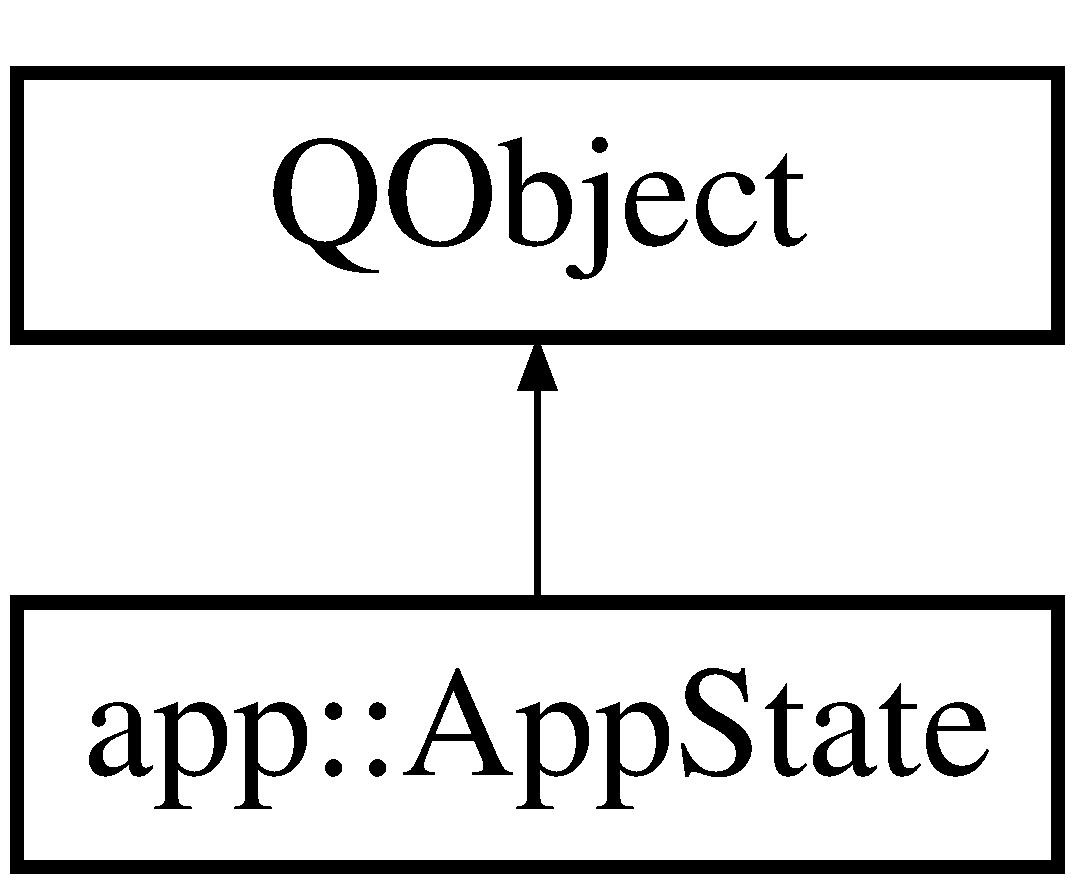
\includegraphics[height=2.000000cm]{classapp_1_1_app_state}
\end{center}
\end{figure}
\subsection*{Public Types}
\begin{DoxyCompactItemize}
\item 
enum \mbox{\hyperlink{classapp_1_1_app_state_aa641298e5827611da2512591c4a0e966}{Tool}} \{ \mbox{\hyperlink{classapp_1_1_app_state_aa641298e5827611da2512591c4a0e966aa9aa485597b649cc4db197bb200d95dc}{R\+E\+C\+T\+A\+N\+G\+LE}}, 
\mbox{\hyperlink{classapp_1_1_app_state_aa641298e5827611da2512591c4a0e966a112f1d74b0e0ce3d3284a1335a8f55e6}{C\+I\+R\+C\+LE}}, 
\mbox{\hyperlink{classapp_1_1_app_state_aa641298e5827611da2512591c4a0e966a11b967f8a13bcf8ea0e5b4d068b62094}{S\+Q\+U\+A\+RE}}
 \}
\begin{DoxyCompactList}\small\item\em Tool Enum, Possible shapes. \end{DoxyCompactList}\end{DoxyCompactItemize}
\subsection*{Public Slots}
\begin{DoxyCompactItemize}
\item 
void \mbox{\hyperlink{classapp_1_1_app_state_a65d839605a7f6926bc2d46534b20ec8c}{set\+Selected\+Tool}} (\mbox{\hyperlink{classapp_1_1_app_state_aa641298e5827611da2512591c4a0e966}{Tool}} seleccted\+Tool)
\item 
void \mbox{\hyperlink{classapp_1_1_app_state_a3e246deb0691d9b0692da546e65c707c}{set\+Selected\+Color}} (Q\+Color \mbox{\hyperlink{classapp_1_1_app_state_a05c87aa8f14b8689902f8aaa363adcc7}{selected\+Color}})
\item 
void \mbox{\hyperlink{classapp_1_1_app_state_ad0d673e923cf52550d08741ccfabbccf}{set\+Selected\+Heigth}} (qreal \mbox{\hyperlink{classapp_1_1_app_state_aaddaf0dbd8c0c99c41968ac6a92709d8}{selected\+Height}})
\item 
void \mbox{\hyperlink{classapp_1_1_app_state_aa7d1b711173cc1ccce7b747d493aa549}{set\+Selected\+Width}} (qreal \mbox{\hyperlink{classapp_1_1_app_state_a31ce013025c446fc7c9f807fe17c0375}{selected\+Width}})
\item 
void \mbox{\hyperlink{classapp_1_1_app_state_a2ce0da74b5c7c3e307f0b55ca6783c58}{set\+Selected\+Position}} (Q\+Point \mbox{\hyperlink{classapp_1_1_app_state_a9fda13b0d9336fc80b2913453694d4c6}{selected\+Position}})
\item 
void \mbox{\hyperlink{classapp_1_1_app_state_a14b1cf39be8be49f16baa526949fd564}{set\+Selected\+Shape}} (Q\+Abstract\+Graphics\+Shape\+Item $\ast$\mbox{\hyperlink{classapp_1_1_app_state_aef0851d3a3c35bb860e43f5dc682d9a7}{selected\+Shape}})
\end{DoxyCompactItemize}
\subsection*{Signals}
\begin{DoxyCompactItemize}
\item 
void \mbox{\hyperlink{classapp_1_1_app_state_a7c4e871a2fece275654f1dfa4b963119}{selected\+Tool\+Changed}} (\mbox{\hyperlink{classapp_1_1_app_state_aa641298e5827611da2512591c4a0e966}{Tool}})
\item 
void \mbox{\hyperlink{classapp_1_1_app_state_afad9c73d20d2ebe623a877eb9558570f}{selected\+Width\+Changed}} (qreal)
\item 
void \mbox{\hyperlink{classapp_1_1_app_state_a7780247f4dc81e62f9a12c6f4c733385}{selected\+Height\+Changed}} (qreal)
\end{DoxyCompactItemize}
\subsection*{Public Member Functions}
\begin{DoxyCompactItemize}
\item 
\mbox{\hyperlink{classapp_1_1_app_state_a467580496a0d9b8641373c52b4cb3918}{App\+State}} ()
\item 
\mbox{\hyperlink{classapp_1_1_app_state_aa641298e5827611da2512591c4a0e966}{Tool}} \mbox{\hyperlink{classapp_1_1_app_state_adcdc7d3fa11e8aecd45baf4f4eb75ef7}{selected\+Tool}} ()
\item 
Q\+Color \mbox{\hyperlink{classapp_1_1_app_state_a05c87aa8f14b8689902f8aaa363adcc7}{selected\+Color}} ()
\item 
qreal \mbox{\hyperlink{classapp_1_1_app_state_aaddaf0dbd8c0c99c41968ac6a92709d8}{selected\+Height}} ()
\item 
qreal \mbox{\hyperlink{classapp_1_1_app_state_a31ce013025c446fc7c9f807fe17c0375}{selected\+Width}} ()
\item 
Q\+Point \mbox{\hyperlink{classapp_1_1_app_state_a9fda13b0d9336fc80b2913453694d4c6}{selected\+Position}} ()
\item 
Q\+Abstract\+Graphics\+Shape\+Item $\ast$ \mbox{\hyperlink{classapp_1_1_app_state_aef0851d3a3c35bb860e43f5dc682d9a7}{selected\+Shape}} ()
\end{DoxyCompactItemize}
\subsection*{Private Attributes}
\begin{DoxyCompactItemize}
\item 
\mbox{\hyperlink{classapp_1_1_app_state_aa641298e5827611da2512591c4a0e966}{Tool}} \mbox{\hyperlink{classapp_1_1_app_state_a80f8f7a574b269f73119edd2ed96f192}{m\+\_\+selected\+Tool}}
\begin{DoxyCompactList}\small\item\em Tool of shape. \end{DoxyCompactList}\item 
Q\+Color \mbox{\hyperlink{classapp_1_1_app_state_a5ad9b96983f21e5718f84d1571f15b7b}{m\+\_\+selected\+Color}}
\begin{DoxyCompactList}\small\item\em color of shape \end{DoxyCompactList}\item 
qreal \mbox{\hyperlink{classapp_1_1_app_state_a22f0a67d5db0c430d32306383491d316}{m\+\_\+selected\+Height}} =55
\begin{DoxyCompactList}\small\item\em height of shape \end{DoxyCompactList}\item 
qreal \mbox{\hyperlink{classapp_1_1_app_state_ad90790bef930b14bdee28a7fb2988c85}{m\+\_\+selected\+Width}} =55
\begin{DoxyCompactList}\small\item\em width of shape \end{DoxyCompactList}\item 
Q\+Point \mbox{\hyperlink{classapp_1_1_app_state_a08af1ba9a3d291aa855e84419588db4f}{m\+\_\+selected\+Position}}
\begin{DoxyCompactList}\small\item\em position of shape \end{DoxyCompactList}\item 
Q\+Abstract\+Graphics\+Shape\+Item $\ast$ \mbox{\hyperlink{classapp_1_1_app_state_a02857da24d9d464ea4e1ffcab7f3c5cf}{m\+\_\+selected\+Shape}}
\begin{DoxyCompactList}\small\item\em shape \end{DoxyCompactList}\end{DoxyCompactItemize}


\subsection{Detailed Description}
This Class Stores the state of the application, for Examble the current tool and it Use default values for all member variables. 

\begin{DoxyAuthor}{Author}
Mohamed 
\end{DoxyAuthor}
\begin{DoxyDate}{Date}
04.\+12.\+2018 
\end{DoxyDate}
\begin{DoxyVersion}{Version}
0.\+2 
\end{DoxyVersion}


Definition at line 17 of file appstate.\+h.



\subsection{Member Enumeration Documentation}
\mbox{\Hypertarget{classapp_1_1_app_state_aa641298e5827611da2512591c4a0e966}\label{classapp_1_1_app_state_aa641298e5827611da2512591c4a0e966}} 
\index{app\+::\+App\+State@{app\+::\+App\+State}!Tool@{Tool}}
\index{Tool@{Tool}!app\+::\+App\+State@{app\+::\+App\+State}}
\subsubsection{\texorpdfstring{Tool}{Tool}}
{\footnotesize\ttfamily enum \mbox{\hyperlink{classapp_1_1_app_state_aa641298e5827611da2512591c4a0e966}{app\+::\+App\+State\+::\+Tool}}}



Tool Enum, Possible shapes. 

\begin{DoxyEnumFields}{Enumerator}
\raisebox{\heightof{T}}[0pt][0pt]{\index{R\+E\+C\+T\+A\+N\+G\+LE@{R\+E\+C\+T\+A\+N\+G\+LE}!app\+::\+App\+State@{app\+::\+App\+State}}\index{app\+::\+App\+State@{app\+::\+App\+State}!R\+E\+C\+T\+A\+N\+G\+LE@{R\+E\+C\+T\+A\+N\+G\+LE}}}\mbox{\Hypertarget{classapp_1_1_app_state_aa641298e5827611da2512591c4a0e966aa9aa485597b649cc4db197bb200d95dc}\label{classapp_1_1_app_state_aa641298e5827611da2512591c4a0e966aa9aa485597b649cc4db197bb200d95dc}} 
R\+E\+C\+T\+A\+N\+G\+LE&Rectangle shape. \\
\hline

\raisebox{\heightof{T}}[0pt][0pt]{\index{C\+I\+R\+C\+LE@{C\+I\+R\+C\+LE}!app\+::\+App\+State@{app\+::\+App\+State}}\index{app\+::\+App\+State@{app\+::\+App\+State}!C\+I\+R\+C\+LE@{C\+I\+R\+C\+LE}}}\mbox{\Hypertarget{classapp_1_1_app_state_aa641298e5827611da2512591c4a0e966a112f1d74b0e0ce3d3284a1335a8f55e6}\label{classapp_1_1_app_state_aa641298e5827611da2512591c4a0e966a112f1d74b0e0ce3d3284a1335a8f55e6}} 
C\+I\+R\+C\+LE&Circle shape. \\
\hline

\raisebox{\heightof{T}}[0pt][0pt]{\index{S\+Q\+U\+A\+RE@{S\+Q\+U\+A\+RE}!app\+::\+App\+State@{app\+::\+App\+State}}\index{app\+::\+App\+State@{app\+::\+App\+State}!S\+Q\+U\+A\+RE@{S\+Q\+U\+A\+RE}}}\mbox{\Hypertarget{classapp_1_1_app_state_aa641298e5827611da2512591c4a0e966a11b967f8a13bcf8ea0e5b4d068b62094}\label{classapp_1_1_app_state_aa641298e5827611da2512591c4a0e966a11b967f8a13bcf8ea0e5b4d068b62094}} 
S\+Q\+U\+A\+RE&Square. \\
\hline

\end{DoxyEnumFields}


Definition at line 25 of file appstate.\+h.



\subsection{Constructor \& Destructor Documentation}
\mbox{\Hypertarget{classapp_1_1_app_state_a467580496a0d9b8641373c52b4cb3918}\label{classapp_1_1_app_state_a467580496a0d9b8641373c52b4cb3918}} 
\index{app\+::\+App\+State@{app\+::\+App\+State}!App\+State@{App\+State}}
\index{App\+State@{App\+State}!app\+::\+App\+State@{app\+::\+App\+State}}
\subsubsection{\texorpdfstring{App\+State()}{AppState()}}
{\footnotesize\ttfamily app\+::\+App\+State\+::\+App\+State (\begin{DoxyParamCaption}{ }\end{DoxyParamCaption})}



Definition at line 8 of file appstate.\+cpp.



\subsection{Member Function Documentation}
\mbox{\Hypertarget{classapp_1_1_app_state_a05c87aa8f14b8689902f8aaa363adcc7}\label{classapp_1_1_app_state_a05c87aa8f14b8689902f8aaa363adcc7}} 
\index{app\+::\+App\+State@{app\+::\+App\+State}!selected\+Color@{selected\+Color}}
\index{selected\+Color@{selected\+Color}!app\+::\+App\+State@{app\+::\+App\+State}}
\subsubsection{\texorpdfstring{selected\+Color()}{selectedColor()}}
{\footnotesize\ttfamily Q\+Color app\+::\+App\+State\+::selected\+Color (\begin{DoxyParamCaption}{ }\end{DoxyParamCaption})\hspace{0.3cm}{\ttfamily [inline]}}

Simple getter. \begin{DoxyReturn}{Returns}
m\+\_\+selected\+Color 
\end{DoxyReturn}


Definition at line 90 of file appstate.\+h.

\mbox{\Hypertarget{classapp_1_1_app_state_aaddaf0dbd8c0c99c41968ac6a92709d8}\label{classapp_1_1_app_state_aaddaf0dbd8c0c99c41968ac6a92709d8}} 
\index{app\+::\+App\+State@{app\+::\+App\+State}!selected\+Height@{selected\+Height}}
\index{selected\+Height@{selected\+Height}!app\+::\+App\+State@{app\+::\+App\+State}}
\subsubsection{\texorpdfstring{selected\+Height()}{selectedHeight()}}
{\footnotesize\ttfamily qreal app\+::\+App\+State\+::selected\+Height (\begin{DoxyParamCaption}{ }\end{DoxyParamCaption})\hspace{0.3cm}{\ttfamily [inline]}}

Simple getter. \begin{DoxyReturn}{Returns}
m\+\_\+selected\+Height 
\end{DoxyReturn}


Definition at line 97 of file appstate.\+h.

\mbox{\Hypertarget{classapp_1_1_app_state_a7780247f4dc81e62f9a12c6f4c733385}\label{classapp_1_1_app_state_a7780247f4dc81e62f9a12c6f4c733385}} 
\index{app\+::\+App\+State@{app\+::\+App\+State}!selected\+Height\+Changed@{selected\+Height\+Changed}}
\index{selected\+Height\+Changed@{selected\+Height\+Changed}!app\+::\+App\+State@{app\+::\+App\+State}}
\subsubsection{\texorpdfstring{selected\+Height\+Changed}{selectedHeightChanged}}
{\footnotesize\ttfamily void app\+::\+App\+State\+::selected\+Height\+Changed (\begin{DoxyParamCaption}\item[{qreal}]{ }\end{DoxyParamCaption})\hspace{0.3cm}{\ttfamily [signal]}}

\mbox{\Hypertarget{classapp_1_1_app_state_a9fda13b0d9336fc80b2913453694d4c6}\label{classapp_1_1_app_state_a9fda13b0d9336fc80b2913453694d4c6}} 
\index{app\+::\+App\+State@{app\+::\+App\+State}!selected\+Position@{selected\+Position}}
\index{selected\+Position@{selected\+Position}!app\+::\+App\+State@{app\+::\+App\+State}}
\subsubsection{\texorpdfstring{selected\+Position()}{selectedPosition()}}
{\footnotesize\ttfamily Q\+Point app\+::\+App\+State\+::selected\+Position (\begin{DoxyParamCaption}{ }\end{DoxyParamCaption})\hspace{0.3cm}{\ttfamily [inline]}}

Simple getter. \begin{DoxyReturn}{Returns}
m\+\_\+selected\+Position 
\end{DoxyReturn}


Definition at line 111 of file appstate.\+h.

\mbox{\Hypertarget{classapp_1_1_app_state_aef0851d3a3c35bb860e43f5dc682d9a7}\label{classapp_1_1_app_state_aef0851d3a3c35bb860e43f5dc682d9a7}} 
\index{app\+::\+App\+State@{app\+::\+App\+State}!selected\+Shape@{selected\+Shape}}
\index{selected\+Shape@{selected\+Shape}!app\+::\+App\+State@{app\+::\+App\+State}}
\subsubsection{\texorpdfstring{selected\+Shape()}{selectedShape()}}
{\footnotesize\ttfamily Q\+Abstract\+Graphics\+Shape\+Item$\ast$ app\+::\+App\+State\+::selected\+Shape (\begin{DoxyParamCaption}{ }\end{DoxyParamCaption})\hspace{0.3cm}{\ttfamily [inline]}}

Simple getter. \begin{DoxyReturn}{Returns}
m\+\_\+selected\+Shape 
\end{DoxyReturn}


Definition at line 118 of file appstate.\+h.

\mbox{\Hypertarget{classapp_1_1_app_state_adcdc7d3fa11e8aecd45baf4f4eb75ef7}\label{classapp_1_1_app_state_adcdc7d3fa11e8aecd45baf4f4eb75ef7}} 
\index{app\+::\+App\+State@{app\+::\+App\+State}!selected\+Tool@{selected\+Tool}}
\index{selected\+Tool@{selected\+Tool}!app\+::\+App\+State@{app\+::\+App\+State}}
\subsubsection{\texorpdfstring{selected\+Tool()}{selectedTool()}}
{\footnotesize\ttfamily \mbox{\hyperlink{classapp_1_1_app_state_aa641298e5827611da2512591c4a0e966}{Tool}} app\+::\+App\+State\+::selected\+Tool (\begin{DoxyParamCaption}{ }\end{DoxyParamCaption})\hspace{0.3cm}{\ttfamily [inline]}}

Simple getter \begin{DoxyReturn}{Returns}
m\+\_\+selected\+Tool 
\end{DoxyReturn}


Definition at line 83 of file appstate.\+h.

\mbox{\Hypertarget{classapp_1_1_app_state_a7c4e871a2fece275654f1dfa4b963119}\label{classapp_1_1_app_state_a7c4e871a2fece275654f1dfa4b963119}} 
\index{app\+::\+App\+State@{app\+::\+App\+State}!selected\+Tool\+Changed@{selected\+Tool\+Changed}}
\index{selected\+Tool\+Changed@{selected\+Tool\+Changed}!app\+::\+App\+State@{app\+::\+App\+State}}
\subsubsection{\texorpdfstring{selected\+Tool\+Changed}{selectedToolChanged}}
{\footnotesize\ttfamily void app\+::\+App\+State\+::selected\+Tool\+Changed (\begin{DoxyParamCaption}\item[{\mbox{\hyperlink{classapp_1_1_app_state_aa641298e5827611da2512591c4a0e966}{Tool}}}]{ }\end{DoxyParamCaption})\hspace{0.3cm}{\ttfamily [signal]}}

\mbox{\Hypertarget{classapp_1_1_app_state_a31ce013025c446fc7c9f807fe17c0375}\label{classapp_1_1_app_state_a31ce013025c446fc7c9f807fe17c0375}} 
\index{app\+::\+App\+State@{app\+::\+App\+State}!selected\+Width@{selected\+Width}}
\index{selected\+Width@{selected\+Width}!app\+::\+App\+State@{app\+::\+App\+State}}
\subsubsection{\texorpdfstring{selected\+Width()}{selectedWidth()}}
{\footnotesize\ttfamily qreal app\+::\+App\+State\+::selected\+Width (\begin{DoxyParamCaption}{ }\end{DoxyParamCaption})\hspace{0.3cm}{\ttfamily [inline]}}

Simple getter. \begin{DoxyReturn}{Returns}
m\+\_\+selected\+Width 
\end{DoxyReturn}


Definition at line 104 of file appstate.\+h.

\mbox{\Hypertarget{classapp_1_1_app_state_afad9c73d20d2ebe623a877eb9558570f}\label{classapp_1_1_app_state_afad9c73d20d2ebe623a877eb9558570f}} 
\index{app\+::\+App\+State@{app\+::\+App\+State}!selected\+Width\+Changed@{selected\+Width\+Changed}}
\index{selected\+Width\+Changed@{selected\+Width\+Changed}!app\+::\+App\+State@{app\+::\+App\+State}}
\subsubsection{\texorpdfstring{selected\+Width\+Changed}{selectedWidthChanged}}
{\footnotesize\ttfamily void app\+::\+App\+State\+::selected\+Width\+Changed (\begin{DoxyParamCaption}\item[{qreal}]{ }\end{DoxyParamCaption})\hspace{0.3cm}{\ttfamily [signal]}}

\mbox{\Hypertarget{classapp_1_1_app_state_a3e246deb0691d9b0692da546e65c707c}\label{classapp_1_1_app_state_a3e246deb0691d9b0692da546e65c707c}} 
\index{app\+::\+App\+State@{app\+::\+App\+State}!set\+Selected\+Color@{set\+Selected\+Color}}
\index{set\+Selected\+Color@{set\+Selected\+Color}!app\+::\+App\+State@{app\+::\+App\+State}}
\subsubsection{\texorpdfstring{set\+Selected\+Color}{setSelectedColor}}
{\footnotesize\ttfamily void app\+::\+App\+State\+::set\+Selected\+Color (\begin{DoxyParamCaption}\item[{Q\+Color}]{selected\+Color }\end{DoxyParamCaption})\hspace{0.3cm}{\ttfamily [inline]}, {\ttfamily [slot]}}

Simple setter for selected\+Color 

Definition at line 53 of file appstate.\+h.

\mbox{\Hypertarget{classapp_1_1_app_state_ad0d673e923cf52550d08741ccfabbccf}\label{classapp_1_1_app_state_ad0d673e923cf52550d08741ccfabbccf}} 
\index{app\+::\+App\+State@{app\+::\+App\+State}!set\+Selected\+Heigth@{set\+Selected\+Heigth}}
\index{set\+Selected\+Heigth@{set\+Selected\+Heigth}!app\+::\+App\+State@{app\+::\+App\+State}}
\subsubsection{\texorpdfstring{set\+Selected\+Heigth}{setSelectedHeigth}}
{\footnotesize\ttfamily void app\+::\+App\+State\+::set\+Selected\+Heigth (\begin{DoxyParamCaption}\item[{qreal}]{selected\+Height }\end{DoxyParamCaption})\hspace{0.3cm}{\ttfamily [slot]}}

Simple setter for selected\+Height 

Definition at line 25 of file appstate.\+cpp.

\mbox{\Hypertarget{classapp_1_1_app_state_a2ce0da74b5c7c3e307f0b55ca6783c58}\label{classapp_1_1_app_state_a2ce0da74b5c7c3e307f0b55ca6783c58}} 
\index{app\+::\+App\+State@{app\+::\+App\+State}!set\+Selected\+Position@{set\+Selected\+Position}}
\index{set\+Selected\+Position@{set\+Selected\+Position}!app\+::\+App\+State@{app\+::\+App\+State}}
\subsubsection{\texorpdfstring{set\+Selected\+Position}{setSelectedPosition}}
{\footnotesize\ttfamily void app\+::\+App\+State\+::set\+Selected\+Position (\begin{DoxyParamCaption}\item[{Q\+Point}]{selected\+Position }\end{DoxyParamCaption})\hspace{0.3cm}{\ttfamily [inline]}, {\ttfamily [slot]}}

Simple setter for selected\+Position 

Definition at line 67 of file appstate.\+h.

\mbox{\Hypertarget{classapp_1_1_app_state_a14b1cf39be8be49f16baa526949fd564}\label{classapp_1_1_app_state_a14b1cf39be8be49f16baa526949fd564}} 
\index{app\+::\+App\+State@{app\+::\+App\+State}!set\+Selected\+Shape@{set\+Selected\+Shape}}
\index{set\+Selected\+Shape@{set\+Selected\+Shape}!app\+::\+App\+State@{app\+::\+App\+State}}
\subsubsection{\texorpdfstring{set\+Selected\+Shape}{setSelectedShape}}
{\footnotesize\ttfamily void app\+::\+App\+State\+::set\+Selected\+Shape (\begin{DoxyParamCaption}\item[{Q\+Abstract\+Graphics\+Shape\+Item $\ast$}]{selected\+Shape }\end{DoxyParamCaption})\hspace{0.3cm}{\ttfamily [inline]}, {\ttfamily [slot]}}

Simple setter for selected\+Shape 

Definition at line 73 of file appstate.\+h.

\mbox{\Hypertarget{classapp_1_1_app_state_a65d839605a7f6926bc2d46534b20ec8c}\label{classapp_1_1_app_state_a65d839605a7f6926bc2d46534b20ec8c}} 
\index{app\+::\+App\+State@{app\+::\+App\+State}!set\+Selected\+Tool@{set\+Selected\+Tool}}
\index{set\+Selected\+Tool@{set\+Selected\+Tool}!app\+::\+App\+State@{app\+::\+App\+State}}
\subsubsection{\texorpdfstring{set\+Selected\+Tool}{setSelectedTool}}
{\footnotesize\ttfamily void app\+::\+App\+State\+::set\+Selected\+Tool (\begin{DoxyParamCaption}\item[{\mbox{\hyperlink{classapp_1_1_app_state_aa641298e5827611da2512591c4a0e966}{Tool}}}]{seleccted\+Tool }\end{DoxyParamCaption})\hspace{0.3cm}{\ttfamily [slot]}}

Simple setter for selected\+Tool 

Definition at line 12 of file appstate.\+cpp.

\mbox{\Hypertarget{classapp_1_1_app_state_aa7d1b711173cc1ccce7b747d493aa549}\label{classapp_1_1_app_state_aa7d1b711173cc1ccce7b747d493aa549}} 
\index{app\+::\+App\+State@{app\+::\+App\+State}!set\+Selected\+Width@{set\+Selected\+Width}}
\index{set\+Selected\+Width@{set\+Selected\+Width}!app\+::\+App\+State@{app\+::\+App\+State}}
\subsubsection{\texorpdfstring{set\+Selected\+Width}{setSelectedWidth}}
{\footnotesize\ttfamily void app\+::\+App\+State\+::set\+Selected\+Width (\begin{DoxyParamCaption}\item[{qreal}]{selected\+Width }\end{DoxyParamCaption})\hspace{0.3cm}{\ttfamily [slot]}}

Simple setter for selected\+Width 

Definition at line 19 of file appstate.\+cpp.



\subsection{Member Data Documentation}
\mbox{\Hypertarget{classapp_1_1_app_state_a5ad9b96983f21e5718f84d1571f15b7b}\label{classapp_1_1_app_state_a5ad9b96983f21e5718f84d1571f15b7b}} 
\index{app\+::\+App\+State@{app\+::\+App\+State}!m\+\_\+selected\+Color@{m\+\_\+selected\+Color}}
\index{m\+\_\+selected\+Color@{m\+\_\+selected\+Color}!app\+::\+App\+State@{app\+::\+App\+State}}
\subsubsection{\texorpdfstring{m\+\_\+selected\+Color}{m\_selectedColor}}
{\footnotesize\ttfamily Q\+Color app\+::\+App\+State\+::m\+\_\+selected\+Color\hspace{0.3cm}{\ttfamily [private]}}



color of shape 



Definition at line 39 of file appstate.\+h.

\mbox{\Hypertarget{classapp_1_1_app_state_a22f0a67d5db0c430d32306383491d316}\label{classapp_1_1_app_state_a22f0a67d5db0c430d32306383491d316}} 
\index{app\+::\+App\+State@{app\+::\+App\+State}!m\+\_\+selected\+Height@{m\+\_\+selected\+Height}}
\index{m\+\_\+selected\+Height@{m\+\_\+selected\+Height}!app\+::\+App\+State@{app\+::\+App\+State}}
\subsubsection{\texorpdfstring{m\+\_\+selected\+Height}{m\_selectedHeight}}
{\footnotesize\ttfamily qreal app\+::\+App\+State\+::m\+\_\+selected\+Height =55\hspace{0.3cm}{\ttfamily [private]}}



height of shape 



Definition at line 40 of file appstate.\+h.

\mbox{\Hypertarget{classapp_1_1_app_state_a08af1ba9a3d291aa855e84419588db4f}\label{classapp_1_1_app_state_a08af1ba9a3d291aa855e84419588db4f}} 
\index{app\+::\+App\+State@{app\+::\+App\+State}!m\+\_\+selected\+Position@{m\+\_\+selected\+Position}}
\index{m\+\_\+selected\+Position@{m\+\_\+selected\+Position}!app\+::\+App\+State@{app\+::\+App\+State}}
\subsubsection{\texorpdfstring{m\+\_\+selected\+Position}{m\_selectedPosition}}
{\footnotesize\ttfamily Q\+Point app\+::\+App\+State\+::m\+\_\+selected\+Position\hspace{0.3cm}{\ttfamily [private]}}



position of shape 



Definition at line 42 of file appstate.\+h.

\mbox{\Hypertarget{classapp_1_1_app_state_a02857da24d9d464ea4e1ffcab7f3c5cf}\label{classapp_1_1_app_state_a02857da24d9d464ea4e1ffcab7f3c5cf}} 
\index{app\+::\+App\+State@{app\+::\+App\+State}!m\+\_\+selected\+Shape@{m\+\_\+selected\+Shape}}
\index{m\+\_\+selected\+Shape@{m\+\_\+selected\+Shape}!app\+::\+App\+State@{app\+::\+App\+State}}
\subsubsection{\texorpdfstring{m\+\_\+selected\+Shape}{m\_selectedShape}}
{\footnotesize\ttfamily Q\+Abstract\+Graphics\+Shape\+Item$\ast$ app\+::\+App\+State\+::m\+\_\+selected\+Shape\hspace{0.3cm}{\ttfamily [private]}}



shape 



Definition at line 43 of file appstate.\+h.

\mbox{\Hypertarget{classapp_1_1_app_state_a80f8f7a574b269f73119edd2ed96f192}\label{classapp_1_1_app_state_a80f8f7a574b269f73119edd2ed96f192}} 
\index{app\+::\+App\+State@{app\+::\+App\+State}!m\+\_\+selected\+Tool@{m\+\_\+selected\+Tool}}
\index{m\+\_\+selected\+Tool@{m\+\_\+selected\+Tool}!app\+::\+App\+State@{app\+::\+App\+State}}
\subsubsection{\texorpdfstring{m\+\_\+selected\+Tool}{m\_selectedTool}}
{\footnotesize\ttfamily \mbox{\hyperlink{classapp_1_1_app_state_aa641298e5827611da2512591c4a0e966}{Tool}} app\+::\+App\+State\+::m\+\_\+selected\+Tool\hspace{0.3cm}{\ttfamily [private]}}



Tool of shape. 



Definition at line 38 of file appstate.\+h.

\mbox{\Hypertarget{classapp_1_1_app_state_ad90790bef930b14bdee28a7fb2988c85}\label{classapp_1_1_app_state_ad90790bef930b14bdee28a7fb2988c85}} 
\index{app\+::\+App\+State@{app\+::\+App\+State}!m\+\_\+selected\+Width@{m\+\_\+selected\+Width}}
\index{m\+\_\+selected\+Width@{m\+\_\+selected\+Width}!app\+::\+App\+State@{app\+::\+App\+State}}
\subsubsection{\texorpdfstring{m\+\_\+selected\+Width}{m\_selectedWidth}}
{\footnotesize\ttfamily qreal app\+::\+App\+State\+::m\+\_\+selected\+Width =55\hspace{0.3cm}{\ttfamily [private]}}



width of shape 



Definition at line 41 of file appstate.\+h.



The documentation for this class was generated from the following files\+:\begin{DoxyCompactItemize}
\item 
\mbox{\hyperlink{appstate_8h}{appstate.\+h}}\item 
\mbox{\hyperlink{appstate_8cpp}{appstate.\+cpp}}\end{DoxyCompactItemize}

\hypertarget{class_circle_dialog}{}\section{Circle\+Dialog Class Reference}
\label{class_circle_dialog}\index{Circle\+Dialog@{Circle\+Dialog}}


this Dialog show The Component to calculate a Area or Circumfernce from Circle using Radius And vice versa.  




{\ttfamily \#include $<$circledialog.\+h$>$}

Inheritance diagram for Circle\+Dialog\+:\begin{figure}[H]
\begin{center}
\leavevmode
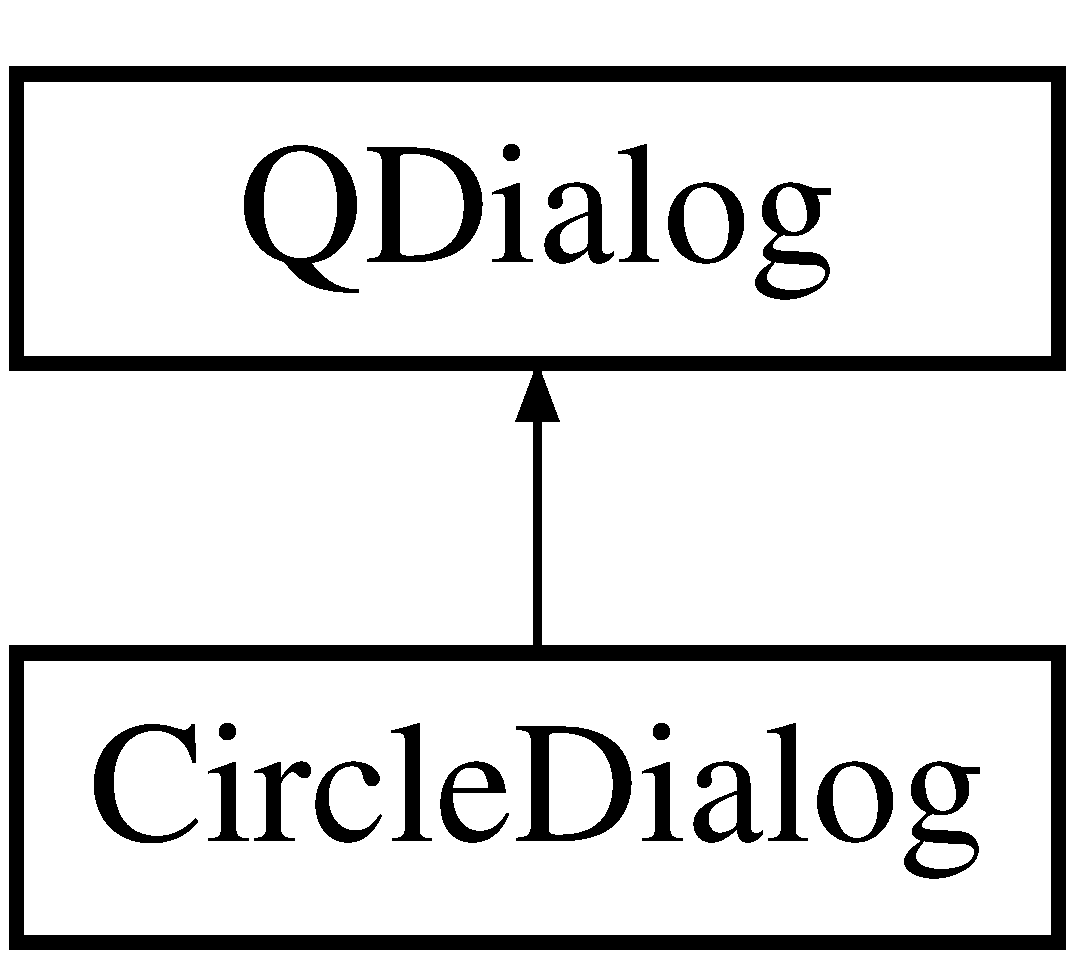
\includegraphics[height=2.000000cm]{class_circle_dialog}
\end{center}
\end{figure}
\subsection*{Public Member Functions}
\begin{DoxyCompactItemize}
\item 
\mbox{\hyperlink{class_circle_dialog_a2ecf57d02624a8b71b87b4c6932b31e7}{Circle\+Dialog}} (Q\+Widget $\ast$parent=nullptr)
\item 
\mbox{\hyperlink{class_circle_dialog_af6f4fa50cf7f1f797060639189a18382}{$\sim$\+Circle\+Dialog}} ()
\end{DoxyCompactItemize}
\subsection*{Private Slots}
\begin{DoxyCompactItemize}
\item 
void \mbox{\hyperlink{class_circle_dialog_a30ff932eb29dc95c4467ba421b5851a8}{on\+\_\+push\+Button\+\_\+\+Area\+\_\+\+Circumferenc\+\_\+clicked}} ()
\begin{DoxyCompactList}\small\item\em on\+\_\+push\+Button\+\_\+\+Area\+\_\+\+Circumferenc\+\_\+clicked This Function calculate the Area and the Circumfernce The Circle using Radius \end{DoxyCompactList}\item 
void \mbox{\hyperlink{class_circle_dialog_ab63c3e021ff34ce5b48c98ec57f40a8e}{on\+\_\+push\+Button\+\_\+\+Radius\+\_\+\+Circumference\+\_\+clicked}} ()
\begin{DoxyCompactList}\small\item\em on\+\_\+push\+Button\+\_\+\+Radius\+\_\+\+Circumference\+\_\+clicked This Function calculate the Radius of The Circle using Circumference \end{DoxyCompactList}\item 
void \mbox{\hyperlink{class_circle_dialog_ad4190e5db5c4d25be7643053b82e0f76}{on\+\_\+push\+Button\+\_\+\+Radius\+\_\+\+Area\+\_\+clicked}} ()
\begin{DoxyCompactList}\small\item\em on\+\_\+push\+Button\+\_\+\+Radius\+\_\+\+Area\+\_\+clicked This Function calculate the Area of The Circle using Radius \end{DoxyCompactList}\end{DoxyCompactItemize}
\subsection*{Private Attributes}
\begin{DoxyCompactItemize}
\item 
Ui\+::\+Circle\+Dialog $\ast$ \mbox{\hyperlink{class_circle_dialog_a44a0e6657fdc9ee80e99a6179e82564a}{ui}}
\end{DoxyCompactItemize}


\subsection{Detailed Description}
this Dialog show The Component to calculate a Area or Circumfernce from Circle using Radius And vice versa. 

\begin{DoxyAuthor}{Author}
Mohamed 
\end{DoxyAuthor}
\begin{DoxyDate}{Date}
22.\+01.\+2018 
\end{DoxyDate}
\begin{DoxyVersion}{Version}
0.\+1 
\end{DoxyVersion}


Definition at line 17 of file circledialog.\+h.



\subsection{Constructor \& Destructor Documentation}
\mbox{\Hypertarget{class_circle_dialog_a2ecf57d02624a8b71b87b4c6932b31e7}\label{class_circle_dialog_a2ecf57d02624a8b71b87b4c6932b31e7}} 
\index{Circle\+Dialog@{Circle\+Dialog}!Circle\+Dialog@{Circle\+Dialog}}
\index{Circle\+Dialog@{Circle\+Dialog}!Circle\+Dialog@{Circle\+Dialog}}
\subsubsection{\texorpdfstring{Circle\+Dialog()}{CircleDialog()}}
{\footnotesize\ttfamily Circle\+Dialog\+::\+Circle\+Dialog (\begin{DoxyParamCaption}\item[{Q\+Widget $\ast$}]{parent = {\ttfamily nullptr} }\end{DoxyParamCaption})\hspace{0.3cm}{\ttfamily [explicit]}}



Definition at line 5 of file Circle\+Dialog.\+cpp.

\mbox{\Hypertarget{class_circle_dialog_af6f4fa50cf7f1f797060639189a18382}\label{class_circle_dialog_af6f4fa50cf7f1f797060639189a18382}} 
\index{Circle\+Dialog@{Circle\+Dialog}!````~Circle\+Dialog@{$\sim$\+Circle\+Dialog}}
\index{````~Circle\+Dialog@{$\sim$\+Circle\+Dialog}!Circle\+Dialog@{Circle\+Dialog}}
\subsubsection{\texorpdfstring{$\sim$\+Circle\+Dialog()}{~CircleDialog()}}
{\footnotesize\ttfamily Circle\+Dialog\+::$\sim$\+Circle\+Dialog (\begin{DoxyParamCaption}{ }\end{DoxyParamCaption})}



Definition at line 12 of file Circle\+Dialog.\+cpp.



\subsection{Member Function Documentation}
\mbox{\Hypertarget{class_circle_dialog_a30ff932eb29dc95c4467ba421b5851a8}\label{class_circle_dialog_a30ff932eb29dc95c4467ba421b5851a8}} 
\index{Circle\+Dialog@{Circle\+Dialog}!on\+\_\+push\+Button\+\_\+\+Area\+\_\+\+Circumferenc\+\_\+clicked@{on\+\_\+push\+Button\+\_\+\+Area\+\_\+\+Circumferenc\+\_\+clicked}}
\index{on\+\_\+push\+Button\+\_\+\+Area\+\_\+\+Circumferenc\+\_\+clicked@{on\+\_\+push\+Button\+\_\+\+Area\+\_\+\+Circumferenc\+\_\+clicked}!Circle\+Dialog@{Circle\+Dialog}}
\subsubsection{\texorpdfstring{on\+\_\+push\+Button\+\_\+\+Area\+\_\+\+Circumferenc\+\_\+clicked}{on\_pushButton\_Area\_Circumferenc\_clicked}}
{\footnotesize\ttfamily void Circle\+Dialog\+::on\+\_\+push\+Button\+\_\+\+Area\+\_\+\+Circumferenc\+\_\+clicked (\begin{DoxyParamCaption}{ }\end{DoxyParamCaption})\hspace{0.3cm}{\ttfamily [private]}, {\ttfamily [slot]}}



on\+\_\+push\+Button\+\_\+\+Area\+\_\+\+Circumferenc\+\_\+clicked This Function calculate the Area and the Circumfernce The Circle using Radius 



Definition at line 18 of file Circle\+Dialog.\+cpp.

\mbox{\Hypertarget{class_circle_dialog_ad4190e5db5c4d25be7643053b82e0f76}\label{class_circle_dialog_ad4190e5db5c4d25be7643053b82e0f76}} 
\index{Circle\+Dialog@{Circle\+Dialog}!on\+\_\+push\+Button\+\_\+\+Radius\+\_\+\+Area\+\_\+clicked@{on\+\_\+push\+Button\+\_\+\+Radius\+\_\+\+Area\+\_\+clicked}}
\index{on\+\_\+push\+Button\+\_\+\+Radius\+\_\+\+Area\+\_\+clicked@{on\+\_\+push\+Button\+\_\+\+Radius\+\_\+\+Area\+\_\+clicked}!Circle\+Dialog@{Circle\+Dialog}}
\subsubsection{\texorpdfstring{on\+\_\+push\+Button\+\_\+\+Radius\+\_\+\+Area\+\_\+clicked}{on\_pushButton\_Radius\_Area\_clicked}}
{\footnotesize\ttfamily void Circle\+Dialog\+::on\+\_\+push\+Button\+\_\+\+Radius\+\_\+\+Area\+\_\+clicked (\begin{DoxyParamCaption}{ }\end{DoxyParamCaption})\hspace{0.3cm}{\ttfamily [private]}, {\ttfamily [slot]}}



on\+\_\+push\+Button\+\_\+\+Radius\+\_\+\+Area\+\_\+clicked This Function calculate the Area of The Circle using Radius 



Definition at line 29 of file Circle\+Dialog.\+cpp.

\mbox{\Hypertarget{class_circle_dialog_ab63c3e021ff34ce5b48c98ec57f40a8e}\label{class_circle_dialog_ab63c3e021ff34ce5b48c98ec57f40a8e}} 
\index{Circle\+Dialog@{Circle\+Dialog}!on\+\_\+push\+Button\+\_\+\+Radius\+\_\+\+Circumference\+\_\+clicked@{on\+\_\+push\+Button\+\_\+\+Radius\+\_\+\+Circumference\+\_\+clicked}}
\index{on\+\_\+push\+Button\+\_\+\+Radius\+\_\+\+Circumference\+\_\+clicked@{on\+\_\+push\+Button\+\_\+\+Radius\+\_\+\+Circumference\+\_\+clicked}!Circle\+Dialog@{Circle\+Dialog}}
\subsubsection{\texorpdfstring{on\+\_\+push\+Button\+\_\+\+Radius\+\_\+\+Circumference\+\_\+clicked}{on\_pushButton\_Radius\_Circumference\_clicked}}
{\footnotesize\ttfamily void Circle\+Dialog\+::on\+\_\+push\+Button\+\_\+\+Radius\+\_\+\+Circumference\+\_\+clicked (\begin{DoxyParamCaption}{ }\end{DoxyParamCaption})\hspace{0.3cm}{\ttfamily [private]}, {\ttfamily [slot]}}



on\+\_\+push\+Button\+\_\+\+Radius\+\_\+\+Circumference\+\_\+clicked This Function calculate the Radius of The Circle using Circumference 



Definition at line 24 of file Circle\+Dialog.\+cpp.



\subsection{Member Data Documentation}
\mbox{\Hypertarget{class_circle_dialog_a44a0e6657fdc9ee80e99a6179e82564a}\label{class_circle_dialog_a44a0e6657fdc9ee80e99a6179e82564a}} 
\index{Circle\+Dialog@{Circle\+Dialog}!ui@{ui}}
\index{ui@{ui}!Circle\+Dialog@{Circle\+Dialog}}
\subsubsection{\texorpdfstring{ui}{ui}}
{\footnotesize\ttfamily Ui\+::\+Circle\+Dialog$\ast$ Circle\+Dialog\+::ui\hspace{0.3cm}{\ttfamily [private]}}



Definition at line 44 of file circledialog.\+h.



The documentation for this class was generated from the following files\+:\begin{DoxyCompactItemize}
\item 
\mbox{\hyperlink{circledialog_8h}{circledialog.\+h}}\item 
\mbox{\hyperlink{_circle_dialog_8cpp}{Circle\+Dialog.\+cpp}}\end{DoxyCompactItemize}

\hypertarget{class_ja___nein___fragen}{}\section{Ja\+\_\+\+Nein\+\_\+\+Fragen Class Reference}
\label{class_ja___nein___fragen}\index{Ja\+\_\+\+Nein\+\_\+\+Fragen@{Ja\+\_\+\+Nein\+\_\+\+Fragen}}


{\ttfamily \#include $<$ja\+\_\+nein\+\_\+fragen.\+h$>$}

Inheritance diagram for Ja\+\_\+\+Nein\+\_\+\+Fragen\+:\begin{figure}[H]
\begin{center}
\leavevmode
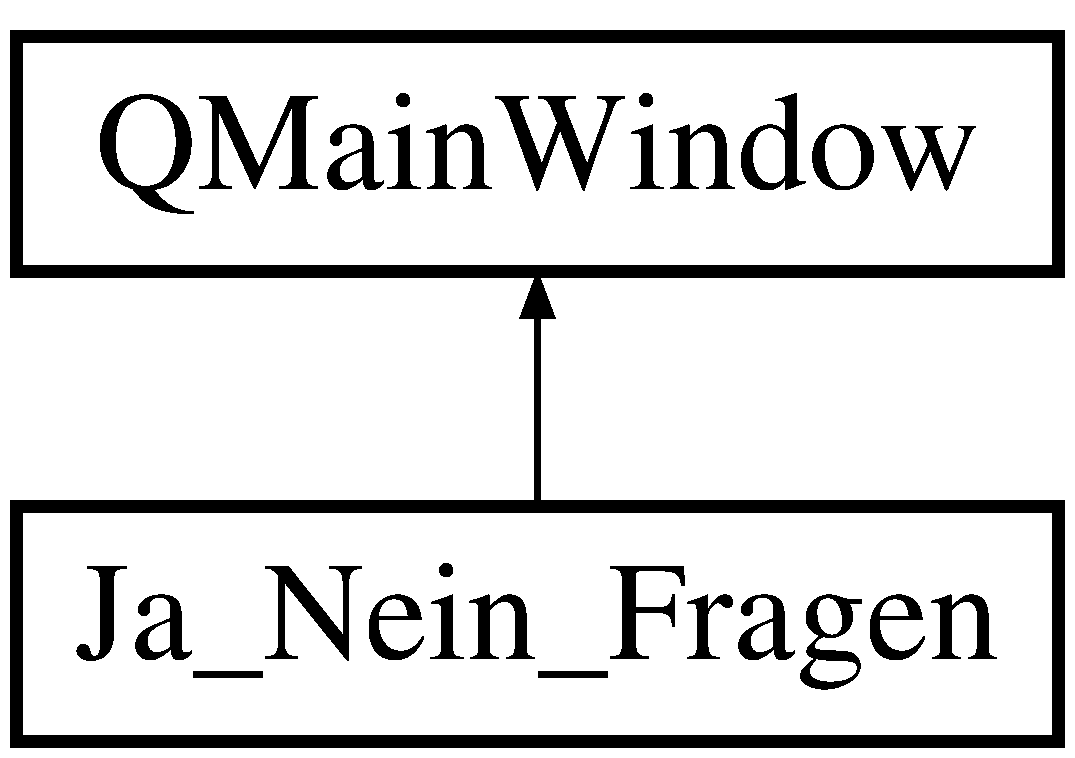
\includegraphics[height=2.000000cm]{class_ja___nein___fragen}
\end{center}
\end{figure}
\subsection*{Public Member Functions}
\begin{DoxyCompactItemize}
\item 
\mbox{\hyperlink{class_ja___nein___fragen_a2a2ae998b3b20083aa5ffbb3437a86f0}{Ja\+\_\+\+Nein\+\_\+\+Fragen}} (Q\+Widget $\ast$parent=nullptr)
\item 
\mbox{\hyperlink{class_ja___nein___fragen_afd95c90bae54f7632d74864f22cdaacc}{$\sim$\+Ja\+\_\+\+Nein\+\_\+\+Fragen}} ()
\end{DoxyCompactItemize}
\subsection*{Private Attributes}
\begin{DoxyCompactItemize}
\item 
Ui\+::\+Ja\+\_\+\+Nein\+\_\+\+Fragen $\ast$ \mbox{\hyperlink{class_ja___nein___fragen_a58aeb9b3bcc790da27ef61440e7ec901}{ui}}
\end{DoxyCompactItemize}


\subsection{Detailed Description}


Definition at line 10 of file ja\+\_\+nein\+\_\+fragen.\+h.



\subsection{Constructor \& Destructor Documentation}
\mbox{\Hypertarget{class_ja___nein___fragen_a2a2ae998b3b20083aa5ffbb3437a86f0}\label{class_ja___nein___fragen_a2a2ae998b3b20083aa5ffbb3437a86f0}} 
\index{Ja\+\_\+\+Nein\+\_\+\+Fragen@{Ja\+\_\+\+Nein\+\_\+\+Fragen}!Ja\+\_\+\+Nein\+\_\+\+Fragen@{Ja\+\_\+\+Nein\+\_\+\+Fragen}}
\index{Ja\+\_\+\+Nein\+\_\+\+Fragen@{Ja\+\_\+\+Nein\+\_\+\+Fragen}!Ja\+\_\+\+Nein\+\_\+\+Fragen@{Ja\+\_\+\+Nein\+\_\+\+Fragen}}
\subsubsection{\texorpdfstring{Ja\+\_\+\+Nein\+\_\+\+Fragen()}{Ja\_Nein\_Fragen()}}
{\footnotesize\ttfamily Ja\+\_\+\+Nein\+\_\+\+Fragen\+::\+Ja\+\_\+\+Nein\+\_\+\+Fragen (\begin{DoxyParamCaption}\item[{Q\+Widget $\ast$}]{parent = {\ttfamily nullptr} }\end{DoxyParamCaption})\hspace{0.3cm}{\ttfamily [explicit]}}



Definition at line 4 of file ja\+\_\+nein\+\_\+fragen.\+cpp.

\mbox{\Hypertarget{class_ja___nein___fragen_afd95c90bae54f7632d74864f22cdaacc}\label{class_ja___nein___fragen_afd95c90bae54f7632d74864f22cdaacc}} 
\index{Ja\+\_\+\+Nein\+\_\+\+Fragen@{Ja\+\_\+\+Nein\+\_\+\+Fragen}!````~Ja\+\_\+\+Nein\+\_\+\+Fragen@{$\sim$\+Ja\+\_\+\+Nein\+\_\+\+Fragen}}
\index{````~Ja\+\_\+\+Nein\+\_\+\+Fragen@{$\sim$\+Ja\+\_\+\+Nein\+\_\+\+Fragen}!Ja\+\_\+\+Nein\+\_\+\+Fragen@{Ja\+\_\+\+Nein\+\_\+\+Fragen}}
\subsubsection{\texorpdfstring{$\sim$\+Ja\+\_\+\+Nein\+\_\+\+Fragen()}{~Ja\_Nein\_Fragen()}}
{\footnotesize\ttfamily Ja\+\_\+\+Nein\+\_\+\+Fragen\+::$\sim$\+Ja\+\_\+\+Nein\+\_\+\+Fragen (\begin{DoxyParamCaption}{ }\end{DoxyParamCaption})}



Definition at line 11 of file ja\+\_\+nein\+\_\+fragen.\+cpp.



\subsection{Member Data Documentation}
\mbox{\Hypertarget{class_ja___nein___fragen_a58aeb9b3bcc790da27ef61440e7ec901}\label{class_ja___nein___fragen_a58aeb9b3bcc790da27ef61440e7ec901}} 
\index{Ja\+\_\+\+Nein\+\_\+\+Fragen@{Ja\+\_\+\+Nein\+\_\+\+Fragen}!ui@{ui}}
\index{ui@{ui}!Ja\+\_\+\+Nein\+\_\+\+Fragen@{Ja\+\_\+\+Nein\+\_\+\+Fragen}}
\subsubsection{\texorpdfstring{ui}{ui}}
{\footnotesize\ttfamily Ui\+::\+Ja\+\_\+\+Nein\+\_\+\+Fragen$\ast$ Ja\+\_\+\+Nein\+\_\+\+Fragen\+::ui\hspace{0.3cm}{\ttfamily [private]}}



Definition at line 19 of file ja\+\_\+nein\+\_\+fragen.\+h.



The documentation for this class was generated from the following files\+:\begin{DoxyCompactItemize}
\item 
\mbox{\hyperlink{ja__nein__fragen_8h}{ja\+\_\+nein\+\_\+fragen.\+h}}\item 
\mbox{\hyperlink{ja__nein__fragen_8cpp}{ja\+\_\+nein\+\_\+fragen.\+cpp}}\end{DoxyCompactItemize}

\hypertarget{class_main_window}{}\section{Main\+Window Class Reference}
\label{class_main_window}\index{Main\+Window@{Main\+Window}}


{\ttfamily \#include $<$mainwindow.\+h$>$}

Inheritance diagram for Main\+Window\+:\begin{figure}[H]
\begin{center}
\leavevmode
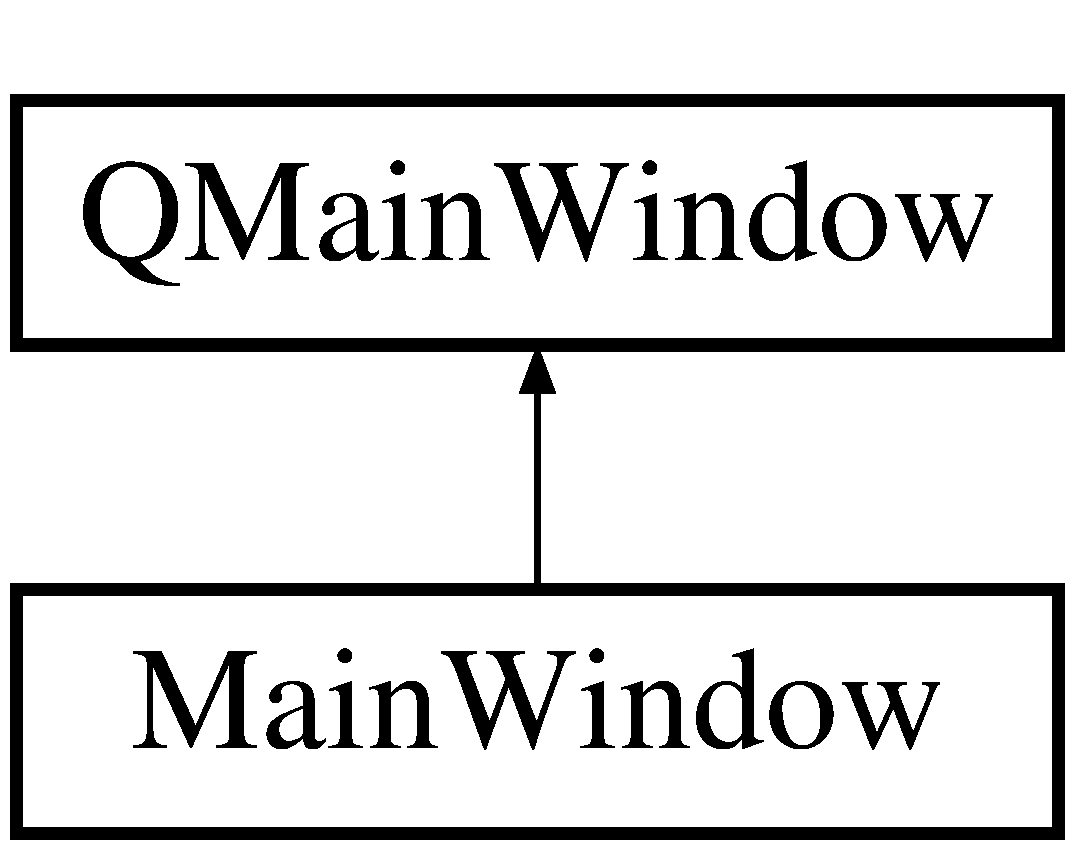
\includegraphics[height=2.000000cm]{class_main_window}
\end{center}
\end{figure}
\subsection*{Public Member Functions}
\begin{DoxyCompactItemize}
\item 
\mbox{\hyperlink{class_main_window_a996c5a2b6f77944776856f08ec30858d}{Main\+Window}} (Q\+Widget $\ast$parent=nullptr)
\item 
\mbox{\hyperlink{class_main_window_ae98d00a93bc118200eeef9f9bba1dba7}{$\sim$\+Main\+Window}} ()
\end{DoxyCompactItemize}
\subsection*{Private Slots}
\begin{DoxyCompactItemize}
\item 
void \mbox{\hyperlink{class_main_window_a1b5f937fcb725434e148ef777c706ae5}{on\+\_\+combo\+Box\+\_\+\+Tool\+\_\+activated}} (const Q\+String \&arg1)
\begin{DoxyCompactList}\small\item\em on\+\_\+combo\+Box\+\_\+\+Tool\+\_\+activated \end{DoxyCompactList}\item 
void \mbox{\hyperlink{class_main_window_abfc114d19ba20fd03b5250ab9bcd6800}{on\+\_\+action\+\_\+ber\+\_\+uns\+\_\+triggered}} ()
\begin{DoxyCompactList}\small\item\em on\+\_\+action\+\_\+ber\+\_\+uns\+\_\+triggered This Function show a Window that have Information about this Programm \end{DoxyCompactList}\item 
void \mbox{\hyperlink{class_main_window_ab3399cf2708da3c92752eee1464b6dac}{on\+\_\+action\+L\+\_\+schen\+\_\+triggered}} ()
\begin{DoxyCompactList}\small\item\em on\+\_\+action\+L\+\_\+schen\+\_\+triggered Removing the current showed Shape in the graphic View \end{DoxyCompactList}\item 
void \mbox{\hyperlink{class_main_window_aba127199cc0e49feec72b68cc89caa73}{on\+\_\+action\+Lernen\+\_\+triggered}} ()
\item 
void \mbox{\hyperlink{class_main_window_a8a59ece8b287b2eea2eba497863e65a2}{on\+\_\+action\+Kreis\+\_\+triggered}} ()
\begin{DoxyCompactList}\small\item\em on\+\_\+action\+Kreis\+\_\+triggered showing Dialog for Circle with Options to calculate \end{DoxyCompactList}\item 
void \mbox{\hyperlink{class_main_window_ada63622ae1c854de4bb80282e490eb14}{on\+\_\+action\+Rechteck\+\_\+triggered}} ()
\begin{DoxyCompactList}\small\item\em on\+\_\+action\+Rechteck\+\_\+triggered showing Dialog for Rectangle with Options to calculate \end{DoxyCompactList}\item 
void \mbox{\hyperlink{class_main_window_a9f891fe4873bb00a7cb186f6d9acb9fe}{on\+\_\+action\+Quadrat\+\_\+triggered}} ()
\begin{DoxyCompactList}\small\item\em on\+\_\+action\+Quadrat\+\_\+triggered showing Dialog for quar with Options to calculate \end{DoxyCompactList}\item 
void \mbox{\hyperlink{class_main_window_a4de79c63c7fa0b8d7c468ac71f20be81}{on\+\_\+push\+Button\+\_\+clicked}} ()
\begin{DoxyCompactList}\small\item\em on\+\_\+push\+Button\+\_\+clicked Close the Main Window \end{DoxyCompactList}\item 
void \mbox{\hyperlink{class_main_window_aa46814868d73e0a0e163c2d4ee855f76}{on\+\_\+action\+\_\+ber\+\_\+\+Kreis\+\_\+triggered}} ()
\begin{DoxyCompactList}\small\item\em on\+\_\+action\+\_\+ber\+\_\+\+Kreis\+\_\+triggered Showing a Dialog with Information about the Circle \end{DoxyCompactList}\item 
void \mbox{\hyperlink{class_main_window_a8581f17d3139d11adedbc775cb17c453}{on\+\_\+action\+\_\+ber\+\_\+\+Rechteck\+\_\+triggered}} ()
\begin{DoxyCompactList}\small\item\em on\+\_\+action\+\_\+ber\+\_\+\+Rechteck\+\_\+triggered Showing a Dialog with Information about the Rectangle \end{DoxyCompactList}\item 
void \mbox{\hyperlink{class_main_window_aae8a9cc8485e71157bc123455a5e4ceb}{on\+\_\+action\+\_\+ber\+\_\+\+Quadrat\+\_\+triggered}} ()
\begin{DoxyCompactList}\small\item\em on\+\_\+action\+\_\+ber\+\_\+\+Quadrat\+\_\+triggered Showing a Dialog with Information about the Square \end{DoxyCompactList}\item 
void \mbox{\hyperlink{class_main_window_aa268869cf5d64f54ee51f41c19a0ee4a}{on\+\_\+action\+Spielen\+\_\+mit\+\_\+\+Lernen\+\_\+triggered}} ()
\begin{DoxyCompactList}\small\item\em on\+\_\+action\+Lernen\+\_\+triggered this Function show a Window that have a True/\+False Quethions for lerning \end{DoxyCompactList}\item 
void \mbox{\hyperlink{class_main_window_a3576ee46f00f0be0850cdc6c7e495ea6}{on\+\_\+actioneine\+\_\+\+Form\+\_\+zeichen\+\_\+triggered}} ()
\begin{DoxyCompactList}\small\item\em on\+\_\+actioneine\+\_\+\+Form\+\_\+zeichen\+\_\+triggered show Dialog that have Information about how to draw a Shape \end{DoxyCompactList}\item 
void \mbox{\hyperlink{class_main_window_a8f8042443101ec9438d82078a16e8aae}{on\+\_\+actioneine\+\_\+\+Form\+\_\+l\+\_\+schen\+\_\+triggered}} ()
\begin{DoxyCompactList}\small\item\em on\+\_\+actioneine\+\_\+\+Form\+\_\+l\+\_\+schen\+\_\+triggered show Dialog that have Information about how to delete a Shape \end{DoxyCompactList}\item 
void \mbox{\hyperlink{class_main_window_aa1da0f626fe8594775c5a43cd5271d53}{on\+\_\+action\+Fl\+\_\+sche\+\_\+des\+\_\+\+Kreises\+\_\+berechnen\+\_\+triggered}} ()
\begin{DoxyCompactList}\small\item\em on\+\_\+action\+Fl\+\_\+sche\+\_\+des\+\_\+\+Kreises\+\_\+berechnen\+\_\+triggered \end{DoxyCompactList}\item 
void \mbox{\hyperlink{class_main_window_a806656e7a0c374ac6e3d42fdf08edc7b}{on\+\_\+action\+Radius\+\_\+des\+\_\+\+Kreises\+\_\+triggered}} ()
\begin{DoxyCompactList}\small\item\em on\+\_\+action\+Radius\+\_\+des\+\_\+\+Kreises\+\_\+triggered show Dialog that have Information about how to calculate the Radius of the Circle using Area or Circmfurance \end{DoxyCompactList}\item 
void \mbox{\hyperlink{class_main_window_aae9811274a2783bdd8c6a4cf76a8f474}{on\+\_\+action\+Fl\+\_\+sche\+\_\+\+Umfang\+\_\+des\+\_\+\+Quadrat\+\_\+triggered}} ()
\begin{DoxyCompactList}\small\item\em on\+\_\+action\+Fl\+\_\+sche\+\_\+\+Umfang\+\_\+des\+\_\+\+Quadrat\+\_\+triggered show Dialog that have Information about how to calculate the Area or the Cicumfurance of Square \end{DoxyCompactList}\item 
void \mbox{\hyperlink{class_main_window_a940ec6db57cf4a86fd6ba85ed258d024}{on\+\_\+action\+Fl\+\_\+sche\+\_\+\+Umfang\+\_\+des\+\_\+\+Rechteck\+\_\+triggered}} ()
\begin{DoxyCompactList}\small\item\em on\+\_\+action\+Fl\+\_\+sche\+\_\+\+Umfang\+\_\+des\+\_\+\+Rechteck\+\_\+triggered show Dialog that have Information about how to calculate the Area or the Cicumfurance of Rectangle \end{DoxyCompactList}\item 
void \mbox{\hyperlink{class_main_window_afb97ac9d597cbe05644fca0581c4d234}{on\+\_\+action\+Seite\+\_\+des\+\_\+\+Quadrates\+\_\+triggered}} ()
\begin{DoxyCompactList}\small\item\em on\+\_\+action\+Seite\+\_\+des\+\_\+\+Quadrates\+\_\+triggered This Function calculate a Side of Squar using Area or Circumference \end{DoxyCompactList}\item 
void \mbox{\hyperlink{class_main_window_a0aaf788d95e063d7320924549ded59aa}{on\+\_\+actiongeometriesche\+\_\+\+Information\+\_\+triggered}} ()
\begin{DoxyCompactList}\small\item\em on\+\_\+actiongeometriesche\+\_\+\+Information\+\_\+triggered show a Dialog that have Information how to get Info. about a spesific Shape \end{DoxyCompactList}\end{DoxyCompactItemize}
\subsection*{Private Attributes}
\begin{DoxyCompactItemize}
\item 
Ui\+::\+Main\+Window $\ast$ \mbox{\hyperlink{class_main_window_a35466a70ed47252a0191168126a352a5}{ui}}
\end{DoxyCompactItemize}


\subsection{Detailed Description}


Definition at line 16 of file mainwindow.\+h.



\subsection{Constructor \& Destructor Documentation}
\mbox{\Hypertarget{class_main_window_a996c5a2b6f77944776856f08ec30858d}\label{class_main_window_a996c5a2b6f77944776856f08ec30858d}} 
\index{Main\+Window@{Main\+Window}!Main\+Window@{Main\+Window}}
\index{Main\+Window@{Main\+Window}!Main\+Window@{Main\+Window}}
\subsubsection{\texorpdfstring{Main\+Window()}{MainWindow()}}
{\footnotesize\ttfamily Main\+Window\+::\+Main\+Window (\begin{DoxyParamCaption}\item[{Q\+Widget $\ast$}]{parent = {\ttfamily nullptr} }\end{DoxyParamCaption})\hspace{0.3cm}{\ttfamily [explicit]}}



Definition at line 11 of file mainwindow.\+cpp.

\mbox{\Hypertarget{class_main_window_ae98d00a93bc118200eeef9f9bba1dba7}\label{class_main_window_ae98d00a93bc118200eeef9f9bba1dba7}} 
\index{Main\+Window@{Main\+Window}!````~Main\+Window@{$\sim$\+Main\+Window}}
\index{````~Main\+Window@{$\sim$\+Main\+Window}!Main\+Window@{Main\+Window}}
\subsubsection{\texorpdfstring{$\sim$\+Main\+Window()}{~MainWindow()}}
{\footnotesize\ttfamily Main\+Window\+::$\sim$\+Main\+Window (\begin{DoxyParamCaption}{ }\end{DoxyParamCaption})}



Definition at line 24 of file mainwindow.\+cpp.



\subsection{Member Function Documentation}
\mbox{\Hypertarget{class_main_window_aa46814868d73e0a0e163c2d4ee855f76}\label{class_main_window_aa46814868d73e0a0e163c2d4ee855f76}} 
\index{Main\+Window@{Main\+Window}!on\+\_\+action\+\_\+ber\+\_\+\+Kreis\+\_\+triggered@{on\+\_\+action\+\_\+ber\+\_\+\+Kreis\+\_\+triggered}}
\index{on\+\_\+action\+\_\+ber\+\_\+\+Kreis\+\_\+triggered@{on\+\_\+action\+\_\+ber\+\_\+\+Kreis\+\_\+triggered}!Main\+Window@{Main\+Window}}
\subsubsection{\texorpdfstring{on\+\_\+action\+\_\+ber\+\_\+\+Kreis\+\_\+triggered}{on\_action\_ber\_Kreis\_triggered}}
{\footnotesize\ttfamily void Main\+Window\+::on\+\_\+action\+\_\+ber\+\_\+\+Kreis\+\_\+triggered (\begin{DoxyParamCaption}{ }\end{DoxyParamCaption})\hspace{0.3cm}{\ttfamily [private]}, {\ttfamily [slot]}}



on\+\_\+action\+\_\+ber\+\_\+\+Kreis\+\_\+triggered Showing a Dialog with Information about the Circle 



Definition at line 154 of file mainwindow.\+cpp.

\mbox{\Hypertarget{class_main_window_aae8a9cc8485e71157bc123455a5e4ceb}\label{class_main_window_aae8a9cc8485e71157bc123455a5e4ceb}} 
\index{Main\+Window@{Main\+Window}!on\+\_\+action\+\_\+ber\+\_\+\+Quadrat\+\_\+triggered@{on\+\_\+action\+\_\+ber\+\_\+\+Quadrat\+\_\+triggered}}
\index{on\+\_\+action\+\_\+ber\+\_\+\+Quadrat\+\_\+triggered@{on\+\_\+action\+\_\+ber\+\_\+\+Quadrat\+\_\+triggered}!Main\+Window@{Main\+Window}}
\subsubsection{\texorpdfstring{on\+\_\+action\+\_\+ber\+\_\+\+Quadrat\+\_\+triggered}{on\_action\_ber\_Quadrat\_triggered}}
{\footnotesize\ttfamily void Main\+Window\+::on\+\_\+action\+\_\+ber\+\_\+\+Quadrat\+\_\+triggered (\begin{DoxyParamCaption}{ }\end{DoxyParamCaption})\hspace{0.3cm}{\ttfamily [private]}, {\ttfamily [slot]}}



on\+\_\+action\+\_\+ber\+\_\+\+Quadrat\+\_\+triggered Showing a Dialog with Information about the Square 



Definition at line 177 of file mainwindow.\+cpp.

\mbox{\Hypertarget{class_main_window_a8581f17d3139d11adedbc775cb17c453}\label{class_main_window_a8581f17d3139d11adedbc775cb17c453}} 
\index{Main\+Window@{Main\+Window}!on\+\_\+action\+\_\+ber\+\_\+\+Rechteck\+\_\+triggered@{on\+\_\+action\+\_\+ber\+\_\+\+Rechteck\+\_\+triggered}}
\index{on\+\_\+action\+\_\+ber\+\_\+\+Rechteck\+\_\+triggered@{on\+\_\+action\+\_\+ber\+\_\+\+Rechteck\+\_\+triggered}!Main\+Window@{Main\+Window}}
\subsubsection{\texorpdfstring{on\+\_\+action\+\_\+ber\+\_\+\+Rechteck\+\_\+triggered}{on\_action\_ber\_Rechteck\_triggered}}
{\footnotesize\ttfamily void Main\+Window\+::on\+\_\+action\+\_\+ber\+\_\+\+Rechteck\+\_\+triggered (\begin{DoxyParamCaption}{ }\end{DoxyParamCaption})\hspace{0.3cm}{\ttfamily [private]}, {\ttfamily [slot]}}



on\+\_\+action\+\_\+ber\+\_\+\+Rechteck\+\_\+triggered Showing a Dialog with Information about the Rectangle 



Definition at line 164 of file mainwindow.\+cpp.

\mbox{\Hypertarget{class_main_window_abfc114d19ba20fd03b5250ab9bcd6800}\label{class_main_window_abfc114d19ba20fd03b5250ab9bcd6800}} 
\index{Main\+Window@{Main\+Window}!on\+\_\+action\+\_\+ber\+\_\+uns\+\_\+triggered@{on\+\_\+action\+\_\+ber\+\_\+uns\+\_\+triggered}}
\index{on\+\_\+action\+\_\+ber\+\_\+uns\+\_\+triggered@{on\+\_\+action\+\_\+ber\+\_\+uns\+\_\+triggered}!Main\+Window@{Main\+Window}}
\subsubsection{\texorpdfstring{on\+\_\+action\+\_\+ber\+\_\+uns\+\_\+triggered}{on\_action\_ber\_uns\_triggered}}
{\footnotesize\ttfamily void Main\+Window\+::on\+\_\+action\+\_\+ber\+\_\+uns\+\_\+triggered (\begin{DoxyParamCaption}{ }\end{DoxyParamCaption})\hspace{0.3cm}{\ttfamily [private]}, {\ttfamily [slot]}}



on\+\_\+action\+\_\+ber\+\_\+uns\+\_\+triggered This Function show a Window that have Information about this Programm 



Definition at line 61 of file mainwindow.\+cpp.

\mbox{\Hypertarget{class_main_window_a8f8042443101ec9438d82078a16e8aae}\label{class_main_window_a8f8042443101ec9438d82078a16e8aae}} 
\index{Main\+Window@{Main\+Window}!on\+\_\+actioneine\+\_\+\+Form\+\_\+l\+\_\+schen\+\_\+triggered@{on\+\_\+actioneine\+\_\+\+Form\+\_\+l\+\_\+schen\+\_\+triggered}}
\index{on\+\_\+actioneine\+\_\+\+Form\+\_\+l\+\_\+schen\+\_\+triggered@{on\+\_\+actioneine\+\_\+\+Form\+\_\+l\+\_\+schen\+\_\+triggered}!Main\+Window@{Main\+Window}}
\subsubsection{\texorpdfstring{on\+\_\+actioneine\+\_\+\+Form\+\_\+l\+\_\+schen\+\_\+triggered}{on\_actioneine\_Form\_l\_schen\_triggered}}
{\footnotesize\ttfamily void Main\+Window\+::on\+\_\+actioneine\+\_\+\+Form\+\_\+l\+\_\+schen\+\_\+triggered (\begin{DoxyParamCaption}{ }\end{DoxyParamCaption})\hspace{0.3cm}{\ttfamily [private]}, {\ttfamily [slot]}}



on\+\_\+actioneine\+\_\+\+Form\+\_\+l\+\_\+schen\+\_\+triggered show Dialog that have Information about how to delete a Shape 



Definition at line 204 of file mainwindow.\+cpp.

\mbox{\Hypertarget{class_main_window_a3576ee46f00f0be0850cdc6c7e495ea6}\label{class_main_window_a3576ee46f00f0be0850cdc6c7e495ea6}} 
\index{Main\+Window@{Main\+Window}!on\+\_\+actioneine\+\_\+\+Form\+\_\+zeichen\+\_\+triggered@{on\+\_\+actioneine\+\_\+\+Form\+\_\+zeichen\+\_\+triggered}}
\index{on\+\_\+actioneine\+\_\+\+Form\+\_\+zeichen\+\_\+triggered@{on\+\_\+actioneine\+\_\+\+Form\+\_\+zeichen\+\_\+triggered}!Main\+Window@{Main\+Window}}
\subsubsection{\texorpdfstring{on\+\_\+actioneine\+\_\+\+Form\+\_\+zeichen\+\_\+triggered}{on\_actioneine\_Form\_zeichen\_triggered}}
{\footnotesize\ttfamily void Main\+Window\+::on\+\_\+actioneine\+\_\+\+Form\+\_\+zeichen\+\_\+triggered (\begin{DoxyParamCaption}{ }\end{DoxyParamCaption})\hspace{0.3cm}{\ttfamily [private]}, {\ttfamily [slot]}}



on\+\_\+actioneine\+\_\+\+Form\+\_\+zeichen\+\_\+triggered show Dialog that have Information about how to draw a Shape 



Definition at line 196 of file mainwindow.\+cpp.

\mbox{\Hypertarget{class_main_window_aa1da0f626fe8594775c5a43cd5271d53}\label{class_main_window_aa1da0f626fe8594775c5a43cd5271d53}} 
\index{Main\+Window@{Main\+Window}!on\+\_\+action\+Fl\+\_\+sche\+\_\+des\+\_\+\+Kreises\+\_\+berechnen\+\_\+triggered@{on\+\_\+action\+Fl\+\_\+sche\+\_\+des\+\_\+\+Kreises\+\_\+berechnen\+\_\+triggered}}
\index{on\+\_\+action\+Fl\+\_\+sche\+\_\+des\+\_\+\+Kreises\+\_\+berechnen\+\_\+triggered@{on\+\_\+action\+Fl\+\_\+sche\+\_\+des\+\_\+\+Kreises\+\_\+berechnen\+\_\+triggered}!Main\+Window@{Main\+Window}}
\subsubsection{\texorpdfstring{on\+\_\+action\+Fl\+\_\+sche\+\_\+des\+\_\+\+Kreises\+\_\+berechnen\+\_\+triggered}{on\_actionFl\_sche\_des\_Kreises\_berechnen\_triggered}}
{\footnotesize\ttfamily void Main\+Window\+::on\+\_\+action\+Fl\+\_\+sche\+\_\+des\+\_\+\+Kreises\+\_\+berechnen\+\_\+triggered (\begin{DoxyParamCaption}{ }\end{DoxyParamCaption})\hspace{0.3cm}{\ttfamily [private]}, {\ttfamily [slot]}}



on\+\_\+action\+Fl\+\_\+sche\+\_\+des\+\_\+\+Kreises\+\_\+berechnen\+\_\+triggered 


\begin{DoxyItemize}
\item show Dialog that have Information about how to calculate the Area or the Cicumfurance 
\end{DoxyItemize}

Definition at line 211 of file mainwindow.\+cpp.

\mbox{\Hypertarget{class_main_window_aae9811274a2783bdd8c6a4cf76a8f474}\label{class_main_window_aae9811274a2783bdd8c6a4cf76a8f474}} 
\index{Main\+Window@{Main\+Window}!on\+\_\+action\+Fl\+\_\+sche\+\_\+\+Umfang\+\_\+des\+\_\+\+Quadrat\+\_\+triggered@{on\+\_\+action\+Fl\+\_\+sche\+\_\+\+Umfang\+\_\+des\+\_\+\+Quadrat\+\_\+triggered}}
\index{on\+\_\+action\+Fl\+\_\+sche\+\_\+\+Umfang\+\_\+des\+\_\+\+Quadrat\+\_\+triggered@{on\+\_\+action\+Fl\+\_\+sche\+\_\+\+Umfang\+\_\+des\+\_\+\+Quadrat\+\_\+triggered}!Main\+Window@{Main\+Window}}
\subsubsection{\texorpdfstring{on\+\_\+action\+Fl\+\_\+sche\+\_\+\+Umfang\+\_\+des\+\_\+\+Quadrat\+\_\+triggered}{on\_actionFl\_sche\_Umfang\_des\_Quadrat\_triggered}}
{\footnotesize\ttfamily void Main\+Window\+::on\+\_\+action\+Fl\+\_\+sche\+\_\+\+Umfang\+\_\+des\+\_\+\+Quadrat\+\_\+triggered (\begin{DoxyParamCaption}{ }\end{DoxyParamCaption})\hspace{0.3cm}{\ttfamily [private]}, {\ttfamily [slot]}}



on\+\_\+action\+Fl\+\_\+sche\+\_\+\+Umfang\+\_\+des\+\_\+\+Quadrat\+\_\+triggered show Dialog that have Information about how to calculate the Area or the Cicumfurance of Square 



Definition at line 227 of file mainwindow.\+cpp.

\mbox{\Hypertarget{class_main_window_a940ec6db57cf4a86fd6ba85ed258d024}\label{class_main_window_a940ec6db57cf4a86fd6ba85ed258d024}} 
\index{Main\+Window@{Main\+Window}!on\+\_\+action\+Fl\+\_\+sche\+\_\+\+Umfang\+\_\+des\+\_\+\+Rechteck\+\_\+triggered@{on\+\_\+action\+Fl\+\_\+sche\+\_\+\+Umfang\+\_\+des\+\_\+\+Rechteck\+\_\+triggered}}
\index{on\+\_\+action\+Fl\+\_\+sche\+\_\+\+Umfang\+\_\+des\+\_\+\+Rechteck\+\_\+triggered@{on\+\_\+action\+Fl\+\_\+sche\+\_\+\+Umfang\+\_\+des\+\_\+\+Rechteck\+\_\+triggered}!Main\+Window@{Main\+Window}}
\subsubsection{\texorpdfstring{on\+\_\+action\+Fl\+\_\+sche\+\_\+\+Umfang\+\_\+des\+\_\+\+Rechteck\+\_\+triggered}{on\_actionFl\_sche\_Umfang\_des\_Rechteck\_triggered}}
{\footnotesize\ttfamily void Main\+Window\+::on\+\_\+action\+Fl\+\_\+sche\+\_\+\+Umfang\+\_\+des\+\_\+\+Rechteck\+\_\+triggered (\begin{DoxyParamCaption}{ }\end{DoxyParamCaption})\hspace{0.3cm}{\ttfamily [private]}, {\ttfamily [slot]}}



on\+\_\+action\+Fl\+\_\+sche\+\_\+\+Umfang\+\_\+des\+\_\+\+Rechteck\+\_\+triggered show Dialog that have Information about how to calculate the Area or the Cicumfurance of Rectangle 



Definition at line 235 of file mainwindow.\+cpp.

\mbox{\Hypertarget{class_main_window_a0aaf788d95e063d7320924549ded59aa}\label{class_main_window_a0aaf788d95e063d7320924549ded59aa}} 
\index{Main\+Window@{Main\+Window}!on\+\_\+actiongeometriesche\+\_\+\+Information\+\_\+triggered@{on\+\_\+actiongeometriesche\+\_\+\+Information\+\_\+triggered}}
\index{on\+\_\+actiongeometriesche\+\_\+\+Information\+\_\+triggered@{on\+\_\+actiongeometriesche\+\_\+\+Information\+\_\+triggered}!Main\+Window@{Main\+Window}}
\subsubsection{\texorpdfstring{on\+\_\+actiongeometriesche\+\_\+\+Information\+\_\+triggered}{on\_actiongeometriesche\_Information\_triggered}}
{\footnotesize\ttfamily void Main\+Window\+::on\+\_\+actiongeometriesche\+\_\+\+Information\+\_\+triggered (\begin{DoxyParamCaption}{ }\end{DoxyParamCaption})\hspace{0.3cm}{\ttfamily [private]}, {\ttfamily [slot]}}



on\+\_\+actiongeometriesche\+\_\+\+Information\+\_\+triggered show a Dialog that have Information how to get Info. about a spesific Shape 



Definition at line 251 of file mainwindow.\+cpp.

\mbox{\Hypertarget{class_main_window_a8a59ece8b287b2eea2eba497863e65a2}\label{class_main_window_a8a59ece8b287b2eea2eba497863e65a2}} 
\index{Main\+Window@{Main\+Window}!on\+\_\+action\+Kreis\+\_\+triggered@{on\+\_\+action\+Kreis\+\_\+triggered}}
\index{on\+\_\+action\+Kreis\+\_\+triggered@{on\+\_\+action\+Kreis\+\_\+triggered}!Main\+Window@{Main\+Window}}
\subsubsection{\texorpdfstring{on\+\_\+action\+Kreis\+\_\+triggered}{on\_actionKreis\_triggered}}
{\footnotesize\ttfamily void Main\+Window\+::on\+\_\+action\+Kreis\+\_\+triggered (\begin{DoxyParamCaption}{ }\end{DoxyParamCaption})\hspace{0.3cm}{\ttfamily [private]}, {\ttfamily [slot]}}



on\+\_\+action\+Kreis\+\_\+triggered showing Dialog for Circle with Options to calculate 



Definition at line 87 of file mainwindow.\+cpp.

\mbox{\Hypertarget{class_main_window_ab3399cf2708da3c92752eee1464b6dac}\label{class_main_window_ab3399cf2708da3c92752eee1464b6dac}} 
\index{Main\+Window@{Main\+Window}!on\+\_\+action\+L\+\_\+schen\+\_\+triggered@{on\+\_\+action\+L\+\_\+schen\+\_\+triggered}}
\index{on\+\_\+action\+L\+\_\+schen\+\_\+triggered@{on\+\_\+action\+L\+\_\+schen\+\_\+triggered}!Main\+Window@{Main\+Window}}
\subsubsection{\texorpdfstring{on\+\_\+action\+L\+\_\+schen\+\_\+triggered}{on\_actionL\_schen\_triggered}}
{\footnotesize\ttfamily void Main\+Window\+::on\+\_\+action\+L\+\_\+schen\+\_\+triggered (\begin{DoxyParamCaption}{ }\end{DoxyParamCaption})\hspace{0.3cm}{\ttfamily [private]}, {\ttfamily [slot]}}



on\+\_\+action\+L\+\_\+schen\+\_\+triggered Removing the current showed Shape in the graphic View 



Definition at line 72 of file mainwindow.\+cpp.

\mbox{\Hypertarget{class_main_window_aba127199cc0e49feec72b68cc89caa73}\label{class_main_window_aba127199cc0e49feec72b68cc89caa73}} 
\index{Main\+Window@{Main\+Window}!on\+\_\+action\+Lernen\+\_\+triggered@{on\+\_\+action\+Lernen\+\_\+triggered}}
\index{on\+\_\+action\+Lernen\+\_\+triggered@{on\+\_\+action\+Lernen\+\_\+triggered}!Main\+Window@{Main\+Window}}
\subsubsection{\texorpdfstring{on\+\_\+action\+Lernen\+\_\+triggered}{on\_actionLernen\_triggered}}
{\footnotesize\ttfamily void Main\+Window\+::on\+\_\+action\+Lernen\+\_\+triggered (\begin{DoxyParamCaption}{ }\end{DoxyParamCaption})\hspace{0.3cm}{\ttfamily [private]}, {\ttfamily [slot]}}



Definition at line 81 of file mainwindow.\+cpp.

\mbox{\Hypertarget{class_main_window_a9f891fe4873bb00a7cb186f6d9acb9fe}\label{class_main_window_a9f891fe4873bb00a7cb186f6d9acb9fe}} 
\index{Main\+Window@{Main\+Window}!on\+\_\+action\+Quadrat\+\_\+triggered@{on\+\_\+action\+Quadrat\+\_\+triggered}}
\index{on\+\_\+action\+Quadrat\+\_\+triggered@{on\+\_\+action\+Quadrat\+\_\+triggered}!Main\+Window@{Main\+Window}}
\subsubsection{\texorpdfstring{on\+\_\+action\+Quadrat\+\_\+triggered}{on\_actionQuadrat\_triggered}}
{\footnotesize\ttfamily void Main\+Window\+::on\+\_\+action\+Quadrat\+\_\+triggered (\begin{DoxyParamCaption}{ }\end{DoxyParamCaption})\hspace{0.3cm}{\ttfamily [private]}, {\ttfamily [slot]}}



on\+\_\+action\+Quadrat\+\_\+triggered showing Dialog for quar with Options to calculate 



Definition at line 103 of file mainwindow.\+cpp.

\mbox{\Hypertarget{class_main_window_a806656e7a0c374ac6e3d42fdf08edc7b}\label{class_main_window_a806656e7a0c374ac6e3d42fdf08edc7b}} 
\index{Main\+Window@{Main\+Window}!on\+\_\+action\+Radius\+\_\+des\+\_\+\+Kreises\+\_\+triggered@{on\+\_\+action\+Radius\+\_\+des\+\_\+\+Kreises\+\_\+triggered}}
\index{on\+\_\+action\+Radius\+\_\+des\+\_\+\+Kreises\+\_\+triggered@{on\+\_\+action\+Radius\+\_\+des\+\_\+\+Kreises\+\_\+triggered}!Main\+Window@{Main\+Window}}
\subsubsection{\texorpdfstring{on\+\_\+action\+Radius\+\_\+des\+\_\+\+Kreises\+\_\+triggered}{on\_actionRadius\_des\_Kreises\_triggered}}
{\footnotesize\ttfamily void Main\+Window\+::on\+\_\+action\+Radius\+\_\+des\+\_\+\+Kreises\+\_\+triggered (\begin{DoxyParamCaption}{ }\end{DoxyParamCaption})\hspace{0.3cm}{\ttfamily [private]}, {\ttfamily [slot]}}



on\+\_\+action\+Radius\+\_\+des\+\_\+\+Kreises\+\_\+triggered show Dialog that have Information about how to calculate the Radius of the Circle using Area or Circmfurance 



Definition at line 219 of file mainwindow.\+cpp.

\mbox{\Hypertarget{class_main_window_ada63622ae1c854de4bb80282e490eb14}\label{class_main_window_ada63622ae1c854de4bb80282e490eb14}} 
\index{Main\+Window@{Main\+Window}!on\+\_\+action\+Rechteck\+\_\+triggered@{on\+\_\+action\+Rechteck\+\_\+triggered}}
\index{on\+\_\+action\+Rechteck\+\_\+triggered@{on\+\_\+action\+Rechteck\+\_\+triggered}!Main\+Window@{Main\+Window}}
\subsubsection{\texorpdfstring{on\+\_\+action\+Rechteck\+\_\+triggered}{on\_actionRechteck\_triggered}}
{\footnotesize\ttfamily void Main\+Window\+::on\+\_\+action\+Rechteck\+\_\+triggered (\begin{DoxyParamCaption}{ }\end{DoxyParamCaption})\hspace{0.3cm}{\ttfamily [private]}, {\ttfamily [slot]}}



on\+\_\+action\+Rechteck\+\_\+triggered showing Dialog for Rectangle with Options to calculate 



Definition at line 95 of file mainwindow.\+cpp.

\mbox{\Hypertarget{class_main_window_afb97ac9d597cbe05644fca0581c4d234}\label{class_main_window_afb97ac9d597cbe05644fca0581c4d234}} 
\index{Main\+Window@{Main\+Window}!on\+\_\+action\+Seite\+\_\+des\+\_\+\+Quadrates\+\_\+triggered@{on\+\_\+action\+Seite\+\_\+des\+\_\+\+Quadrates\+\_\+triggered}}
\index{on\+\_\+action\+Seite\+\_\+des\+\_\+\+Quadrates\+\_\+triggered@{on\+\_\+action\+Seite\+\_\+des\+\_\+\+Quadrates\+\_\+triggered}!Main\+Window@{Main\+Window}}
\subsubsection{\texorpdfstring{on\+\_\+action\+Seite\+\_\+des\+\_\+\+Quadrates\+\_\+triggered}{on\_actionSeite\_des\_Quadrates\_triggered}}
{\footnotesize\ttfamily void Main\+Window\+::on\+\_\+action\+Seite\+\_\+des\+\_\+\+Quadrates\+\_\+triggered (\begin{DoxyParamCaption}{ }\end{DoxyParamCaption})\hspace{0.3cm}{\ttfamily [private]}, {\ttfamily [slot]}}



on\+\_\+action\+Seite\+\_\+des\+\_\+\+Quadrates\+\_\+triggered This Function calculate a Side of Squar using Area or Circumference 



Definition at line 243 of file mainwindow.\+cpp.

\mbox{\Hypertarget{class_main_window_aa268869cf5d64f54ee51f41c19a0ee4a}\label{class_main_window_aa268869cf5d64f54ee51f41c19a0ee4a}} 
\index{Main\+Window@{Main\+Window}!on\+\_\+action\+Spielen\+\_\+mit\+\_\+\+Lernen\+\_\+triggered@{on\+\_\+action\+Spielen\+\_\+mit\+\_\+\+Lernen\+\_\+triggered}}
\index{on\+\_\+action\+Spielen\+\_\+mit\+\_\+\+Lernen\+\_\+triggered@{on\+\_\+action\+Spielen\+\_\+mit\+\_\+\+Lernen\+\_\+triggered}!Main\+Window@{Main\+Window}}
\subsubsection{\texorpdfstring{on\+\_\+action\+Spielen\+\_\+mit\+\_\+\+Lernen\+\_\+triggered}{on\_actionSpielen\_mit\_Lernen\_triggered}}
{\footnotesize\ttfamily void Main\+Window\+::on\+\_\+action\+Spielen\+\_\+mit\+\_\+\+Lernen\+\_\+triggered (\begin{DoxyParamCaption}{ }\end{DoxyParamCaption})\hspace{0.3cm}{\ttfamily [private]}, {\ttfamily [slot]}}



on\+\_\+action\+Lernen\+\_\+triggered this Function show a Window that have a True/\+False Quethions for lerning 



Definition at line 189 of file mainwindow.\+cpp.

\mbox{\Hypertarget{class_main_window_a1b5f937fcb725434e148ef777c706ae5}\label{class_main_window_a1b5f937fcb725434e148ef777c706ae5}} 
\index{Main\+Window@{Main\+Window}!on\+\_\+combo\+Box\+\_\+\+Tool\+\_\+activated@{on\+\_\+combo\+Box\+\_\+\+Tool\+\_\+activated}}
\index{on\+\_\+combo\+Box\+\_\+\+Tool\+\_\+activated@{on\+\_\+combo\+Box\+\_\+\+Tool\+\_\+activated}!Main\+Window@{Main\+Window}}
\subsubsection{\texorpdfstring{on\+\_\+combo\+Box\+\_\+\+Tool\+\_\+activated}{on\_comboBox\_Tool\_activated}}
{\footnotesize\ttfamily void Main\+Window\+::on\+\_\+combo\+Box\+\_\+\+Tool\+\_\+activated (\begin{DoxyParamCaption}\item[{const Q\+String \&}]{arg1 }\end{DoxyParamCaption})\hspace{0.3cm}{\ttfamily [private]}, {\ttfamily [slot]}}



on\+\_\+combo\+Box\+\_\+\+Tool\+\_\+activated 


\begin{DoxyParams}{Parameters}
{\em arg1} & the name of the Shape This Function shows the Boxes for giving Values independing of selected Shape \\
\hline
\end{DoxyParams}


Definition at line 29 of file mainwindow.\+cpp.

\mbox{\Hypertarget{class_main_window_a4de79c63c7fa0b8d7c468ac71f20be81}\label{class_main_window_a4de79c63c7fa0b8d7c468ac71f20be81}} 
\index{Main\+Window@{Main\+Window}!on\+\_\+push\+Button\+\_\+clicked@{on\+\_\+push\+Button\+\_\+clicked}}
\index{on\+\_\+push\+Button\+\_\+clicked@{on\+\_\+push\+Button\+\_\+clicked}!Main\+Window@{Main\+Window}}
\subsubsection{\texorpdfstring{on\+\_\+push\+Button\+\_\+clicked}{on\_pushButton\_clicked}}
{\footnotesize\ttfamily void Main\+Window\+::on\+\_\+push\+Button\+\_\+clicked (\begin{DoxyParamCaption}{ }\end{DoxyParamCaption})\hspace{0.3cm}{\ttfamily [private]}, {\ttfamily [slot]}}



on\+\_\+push\+Button\+\_\+clicked Close the Main Window 



Definition at line 110 of file mainwindow.\+cpp.



\subsection{Member Data Documentation}
\mbox{\Hypertarget{class_main_window_a35466a70ed47252a0191168126a352a5}\label{class_main_window_a35466a70ed47252a0191168126a352a5}} 
\index{Main\+Window@{Main\+Window}!ui@{ui}}
\index{ui@{ui}!Main\+Window@{Main\+Window}}
\subsubsection{\texorpdfstring{ui}{ui}}
{\footnotesize\ttfamily Ui\+::\+Main\+Window$\ast$ Main\+Window\+::ui\hspace{0.3cm}{\ttfamily [private]}}



Definition at line 126 of file mainwindow.\+h.



The documentation for this class was generated from the following files\+:\begin{DoxyCompactItemize}
\item 
\mbox{\hyperlink{mainwindow_8h}{mainwindow.\+h}}\item 
\mbox{\hyperlink{mainwindow_8cpp}{mainwindow.\+cpp}}\end{DoxyCompactItemize}

\hypertarget{class_rectangle_dialog}{}\section{Rectangle\+Dialog Class Reference}
\label{class_rectangle_dialog}\index{Rectangle\+Dialog@{Rectangle\+Dialog}}


The \mbox{\hyperlink{class_rectangle_dialog}{Rectangle\+Dialog}} class show a dialog with options to calculate the area, circumference and side of rectangle.  




{\ttfamily \#include $<$rectangledialog.\+h$>$}

Inheritance diagram for Rectangle\+Dialog\+:\begin{figure}[H]
\begin{center}
\leavevmode
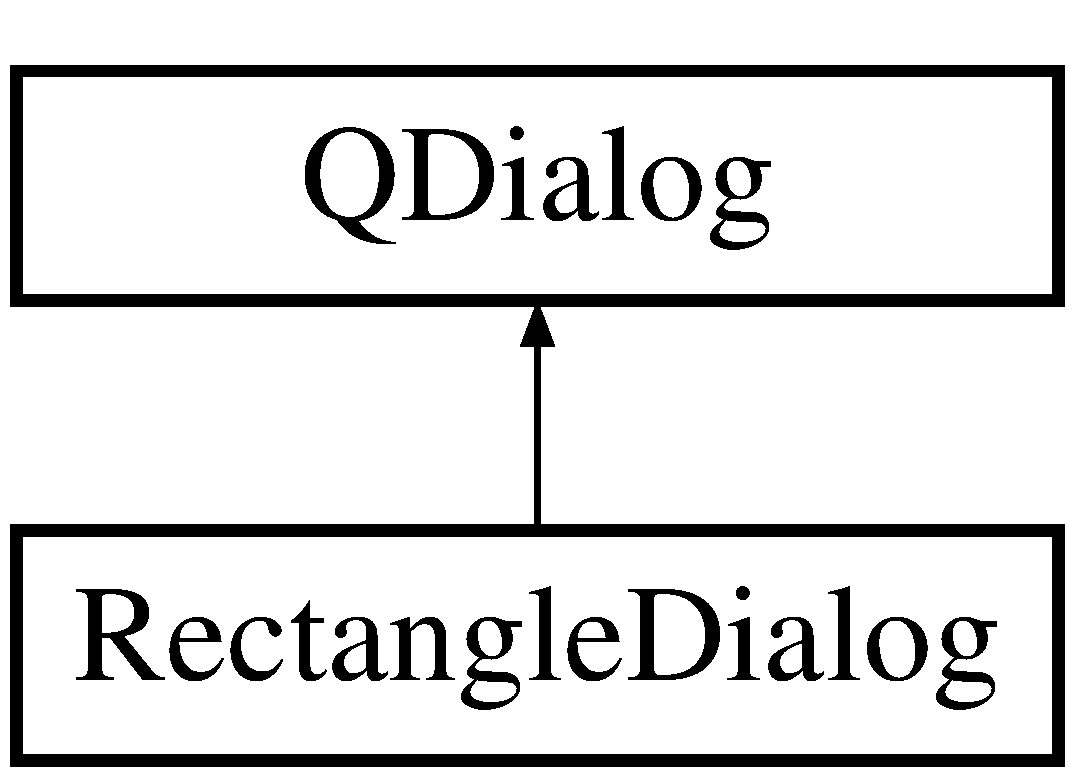
\includegraphics[height=2.000000cm]{class_rectangle_dialog}
\end{center}
\end{figure}
\subsection*{Public Member Functions}
\begin{DoxyCompactItemize}
\item 
\mbox{\hyperlink{class_rectangle_dialog_abe1855a7bfdf24450033fe3c17837db6}{Rectangle\+Dialog}} (Q\+Widget $\ast$parent=nullptr)
\item 
\mbox{\hyperlink{class_rectangle_dialog_a356cf182f6d805c50d5b3c4e97cbae81}{$\sim$\+Rectangle\+Dialog}} ()
\end{DoxyCompactItemize}
\subsection*{Private Slots}
\begin{DoxyCompactItemize}
\item 
void \mbox{\hyperlink{class_rectangle_dialog_a1f4ec776eedd80298bbe6c6f408027c9}{on\+\_\+push\+Button\+\_\+\+Ok\+\_\+clicked}} ()
\begin{DoxyCompactList}\small\item\em on\+\_\+push\+Button\+\_\+\+Ok\+\_\+clicked calculate the Area and the circumference of rectangle \end{DoxyCompactList}\end{DoxyCompactItemize}
\subsection*{Private Attributes}
\begin{DoxyCompactItemize}
\item 
Ui\+::\+Rectangle\+Dialog $\ast$ \mbox{\hyperlink{class_rectangle_dialog_ab65a306d815eaca0c8ff6674f49aea99}{ui}}
\end{DoxyCompactItemize}


\subsection{Detailed Description}
The \mbox{\hyperlink{class_rectangle_dialog}{Rectangle\+Dialog}} class show a dialog with options to calculate the area, circumference and side of rectangle. 

Definition at line 13 of file rectangledialog.\+h.



\subsection{Constructor \& Destructor Documentation}
\mbox{\Hypertarget{class_rectangle_dialog_abe1855a7bfdf24450033fe3c17837db6}\label{class_rectangle_dialog_abe1855a7bfdf24450033fe3c17837db6}} 
\index{Rectangle\+Dialog@{Rectangle\+Dialog}!Rectangle\+Dialog@{Rectangle\+Dialog}}
\index{Rectangle\+Dialog@{Rectangle\+Dialog}!Rectangle\+Dialog@{Rectangle\+Dialog}}
\subsubsection{\texorpdfstring{Rectangle\+Dialog()}{RectangleDialog()}}
{\footnotesize\ttfamily Rectangle\+Dialog\+::\+Rectangle\+Dialog (\begin{DoxyParamCaption}\item[{Q\+Widget $\ast$}]{parent = {\ttfamily nullptr} }\end{DoxyParamCaption})\hspace{0.3cm}{\ttfamily [explicit]}}



Definition at line 4 of file rectangledialog.\+cpp.

\mbox{\Hypertarget{class_rectangle_dialog_a356cf182f6d805c50d5b3c4e97cbae81}\label{class_rectangle_dialog_a356cf182f6d805c50d5b3c4e97cbae81}} 
\index{Rectangle\+Dialog@{Rectangle\+Dialog}!````~Rectangle\+Dialog@{$\sim$\+Rectangle\+Dialog}}
\index{````~Rectangle\+Dialog@{$\sim$\+Rectangle\+Dialog}!Rectangle\+Dialog@{Rectangle\+Dialog}}
\subsubsection{\texorpdfstring{$\sim$\+Rectangle\+Dialog()}{~RectangleDialog()}}
{\footnotesize\ttfamily Rectangle\+Dialog\+::$\sim$\+Rectangle\+Dialog (\begin{DoxyParamCaption}{ }\end{DoxyParamCaption})}



Definition at line 11 of file rectangledialog.\+cpp.



\subsection{Member Function Documentation}
\mbox{\Hypertarget{class_rectangle_dialog_a1f4ec776eedd80298bbe6c6f408027c9}\label{class_rectangle_dialog_a1f4ec776eedd80298bbe6c6f408027c9}} 
\index{Rectangle\+Dialog@{Rectangle\+Dialog}!on\+\_\+push\+Button\+\_\+\+Ok\+\_\+clicked@{on\+\_\+push\+Button\+\_\+\+Ok\+\_\+clicked}}
\index{on\+\_\+push\+Button\+\_\+\+Ok\+\_\+clicked@{on\+\_\+push\+Button\+\_\+\+Ok\+\_\+clicked}!Rectangle\+Dialog@{Rectangle\+Dialog}}
\subsubsection{\texorpdfstring{on\+\_\+push\+Button\+\_\+\+Ok\+\_\+clicked}{on\_pushButton\_Ok\_clicked}}
{\footnotesize\ttfamily void Rectangle\+Dialog\+::on\+\_\+push\+Button\+\_\+\+Ok\+\_\+clicked (\begin{DoxyParamCaption}{ }\end{DoxyParamCaption})\hspace{0.3cm}{\ttfamily [private]}, {\ttfamily [slot]}}



on\+\_\+push\+Button\+\_\+\+Ok\+\_\+clicked calculate the Area and the circumference of rectangle 



Definition at line 16 of file rectangledialog.\+cpp.



\subsection{Member Data Documentation}
\mbox{\Hypertarget{class_rectangle_dialog_ab65a306d815eaca0c8ff6674f49aea99}\label{class_rectangle_dialog_ab65a306d815eaca0c8ff6674f49aea99}} 
\index{Rectangle\+Dialog@{Rectangle\+Dialog}!ui@{ui}}
\index{ui@{ui}!Rectangle\+Dialog@{Rectangle\+Dialog}}
\subsubsection{\texorpdfstring{ui}{ui}}
{\footnotesize\ttfamily Ui\+::\+Rectangle\+Dialog$\ast$ Rectangle\+Dialog\+::ui\hspace{0.3cm}{\ttfamily [private]}}



Definition at line 29 of file rectangledialog.\+h.



The documentation for this class was generated from the following files\+:\begin{DoxyCompactItemize}
\item 
\mbox{\hyperlink{rectangledialog_8h}{rectangledialog.\+h}}\item 
\mbox{\hyperlink{rectangledialog_8cpp}{rectangledialog.\+cpp}}\end{DoxyCompactItemize}

\hypertarget{class_scene}{}\section{Scene Class Reference}
\label{class_scene}\index{Scene@{Scene}}


{\ttfamily \#include $<$scene.\+h$>$}

Inheritance diagram for Scene\+:\begin{figure}[H]
\begin{center}
\leavevmode
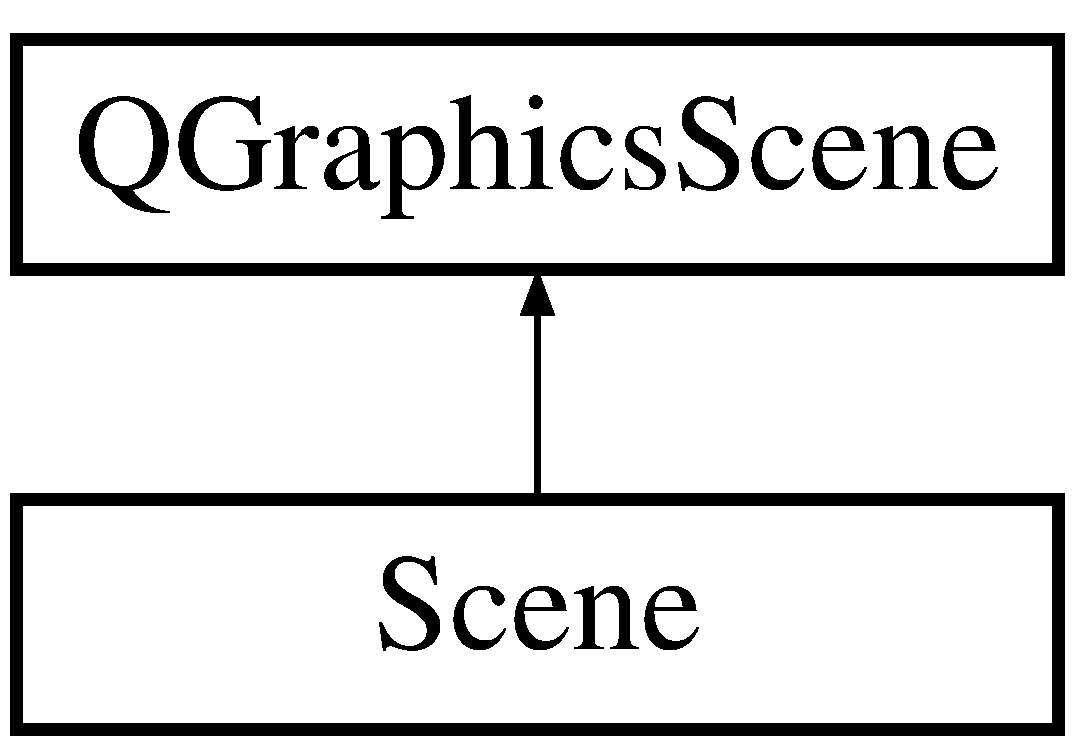
\includegraphics[height=2.000000cm]{class_scene}
\end{center}
\end{figure}
\subsection*{Signals}
\begin{DoxyCompactItemize}
\item 
bool \mbox{\hyperlink{class_scene_a393b0ed4e907779249e2857d3b93a5f1}{mouse\+Press}} (bool has\+Been\+Pressed)
\end{DoxyCompactItemize}
\subsection*{Public Member Functions}
\begin{DoxyCompactItemize}
\item 
\mbox{\hyperlink{class_scene_ad10176d75a9cc0da56626f682d083507}{Scene}} ()
\end{DoxyCompactItemize}
\subsection*{Protected Member Functions}
\begin{DoxyCompactItemize}
\item 
void \mbox{\hyperlink{class_scene_af86554e49d701f3fe9f0ac4f568f7113}{mouse\+Press\+Event}} (Q\+Mouse\+Event $\ast$event)
\end{DoxyCompactItemize}


\subsection{Detailed Description}


Definition at line 6 of file scene.\+h.



\subsection{Constructor \& Destructor Documentation}
\mbox{\Hypertarget{class_scene_ad10176d75a9cc0da56626f682d083507}\label{class_scene_ad10176d75a9cc0da56626f682d083507}} 
\index{Scene@{Scene}!Scene@{Scene}}
\index{Scene@{Scene}!Scene@{Scene}}
\subsubsection{\texorpdfstring{Scene()}{Scene()}}
{\footnotesize\ttfamily Scene\+::\+Scene (\begin{DoxyParamCaption}{ }\end{DoxyParamCaption})}



Definition at line 3 of file scene.\+cpp.



\subsection{Member Function Documentation}
\mbox{\Hypertarget{class_scene_a393b0ed4e907779249e2857d3b93a5f1}\label{class_scene_a393b0ed4e907779249e2857d3b93a5f1}} 
\index{Scene@{Scene}!mouse\+Press@{mouse\+Press}}
\index{mouse\+Press@{mouse\+Press}!Scene@{Scene}}
\subsubsection{\texorpdfstring{mouse\+Press}{mousePress}}
{\footnotesize\ttfamily bool Scene\+::mouse\+Press (\begin{DoxyParamCaption}\item[{bool}]{has\+Been\+Pressed }\end{DoxyParamCaption})\hspace{0.3cm}{\ttfamily [signal]}}

\mbox{\Hypertarget{class_scene_af86554e49d701f3fe9f0ac4f568f7113}\label{class_scene_af86554e49d701f3fe9f0ac4f568f7113}} 
\index{Scene@{Scene}!mouse\+Press\+Event@{mouse\+Press\+Event}}
\index{mouse\+Press\+Event@{mouse\+Press\+Event}!Scene@{Scene}}
\subsubsection{\texorpdfstring{mouse\+Press\+Event()}{mousePressEvent()}}
{\footnotesize\ttfamily void Scene\+::mouse\+Press\+Event (\begin{DoxyParamCaption}\item[{Q\+Mouse\+Event $\ast$}]{event }\end{DoxyParamCaption})\hspace{0.3cm}{\ttfamily [protected]}}



Definition at line 8 of file scene.\+cpp.



The documentation for this class was generated from the following files\+:\begin{DoxyCompactItemize}
\item 
\mbox{\hyperlink{scene_8h}{scene.\+h}}\item 
\mbox{\hyperlink{scene_8cpp}{scene.\+cpp}}\end{DoxyCompactItemize}

\hypertarget{class_square_dialog}{}\section{Square\+Dialog Class Reference}
\label{class_square_dialog}\index{Square\+Dialog@{Square\+Dialog}}


The \mbox{\hyperlink{class_square_dialog}{Square\+Dialog}} class show a dialog with options to calculate the Area, circumference und side of the square.  




{\ttfamily \#include $<$squaredialog.\+h$>$}

Inheritance diagram for Square\+Dialog\+:\begin{figure}[H]
\begin{center}
\leavevmode
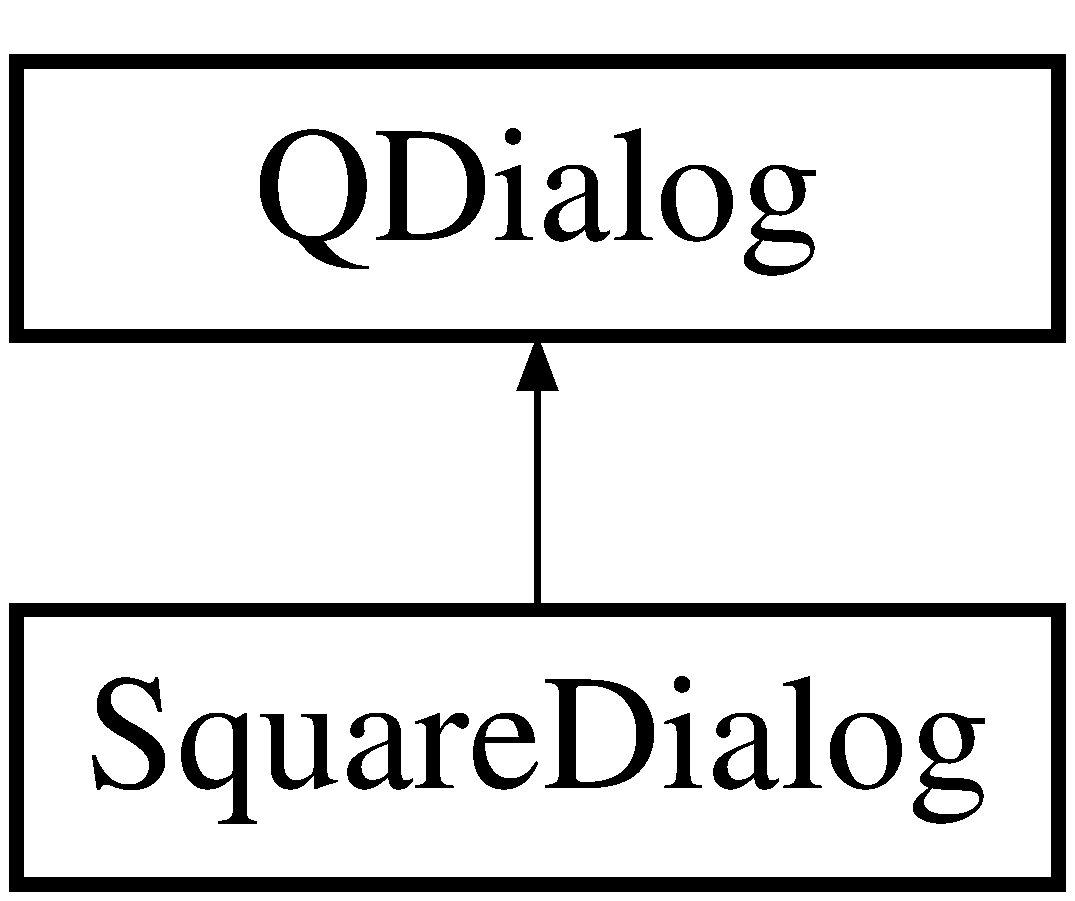
\includegraphics[height=2.000000cm]{class_square_dialog}
\end{center}
\end{figure}
\subsection*{Public Member Functions}
\begin{DoxyCompactItemize}
\item 
\mbox{\hyperlink{class_square_dialog_a091517384d35fe4fbc444ed34a6ba303}{Square\+Dialog}} (Q\+Widget $\ast$parent=nullptr)
\item 
\mbox{\hyperlink{class_square_dialog_a8129e6dc415aea3fca385ac775e32c71}{$\sim$\+Square\+Dialog}} ()
\end{DoxyCompactItemize}
\subsection*{Private Slots}
\begin{DoxyCompactItemize}
\item 
void \mbox{\hyperlink{class_square_dialog_ae51403bfd6b525bb22a857db7ef8cf89}{on\+\_\+push\+Button\+\_\+clicked}} ()
\begin{DoxyCompactList}\small\item\em on\+\_\+push\+Button\+\_\+clicked calculate the Area and the circumference of square \end{DoxyCompactList}\item 
void \mbox{\hyperlink{class_square_dialog_a8cc8d7c0933edc70f88f10e947f9e106}{on\+\_\+push\+Button\+\_\+\+Side\+\_\+\+Circ\+\_\+\+\_\+clicked}} ()
\begin{DoxyCompactList}\small\item\em on\+\_\+push\+Button\+\_\+\+Side\+\_\+\+Circ\+\_\+\+\_\+clicked calculate the side of square using the circumference \end{DoxyCompactList}\item 
void \mbox{\hyperlink{class_square_dialog_a3e51ec196b9d3b5e61bcf177999f05f5}{on\+\_\+push\+Button\+\_\+\+Side\+\_\+\+Area\+\_\+clicked}} ()
\begin{DoxyCompactList}\small\item\em on\+\_\+push\+Button\+\_\+\+Side\+\_\+\+Area\+\_\+clicked calculate the side of square using the Area \end{DoxyCompactList}\end{DoxyCompactItemize}
\subsection*{Private Attributes}
\begin{DoxyCompactItemize}
\item 
Ui\+::\+Square\+Dialog $\ast$ \mbox{\hyperlink{class_square_dialog_a2359f63a0ab0e9d7062b0ff2e60a7e96}{ui}}
\end{DoxyCompactItemize}


\subsection{Detailed Description}
The \mbox{\hyperlink{class_square_dialog}{Square\+Dialog}} class show a dialog with options to calculate the Area, circumference und side of the square. 

Definition at line 14 of file squaredialog.\+h.



\subsection{Constructor \& Destructor Documentation}
\mbox{\Hypertarget{class_square_dialog_a091517384d35fe4fbc444ed34a6ba303}\label{class_square_dialog_a091517384d35fe4fbc444ed34a6ba303}} 
\index{Square\+Dialog@{Square\+Dialog}!Square\+Dialog@{Square\+Dialog}}
\index{Square\+Dialog@{Square\+Dialog}!Square\+Dialog@{Square\+Dialog}}
\subsubsection{\texorpdfstring{Square\+Dialog()}{SquareDialog()}}
{\footnotesize\ttfamily Square\+Dialog\+::\+Square\+Dialog (\begin{DoxyParamCaption}\item[{Q\+Widget $\ast$}]{parent = {\ttfamily nullptr} }\end{DoxyParamCaption})\hspace{0.3cm}{\ttfamily [explicit]}}



Definition at line 4 of file squaredialog.\+cpp.

\mbox{\Hypertarget{class_square_dialog_a8129e6dc415aea3fca385ac775e32c71}\label{class_square_dialog_a8129e6dc415aea3fca385ac775e32c71}} 
\index{Square\+Dialog@{Square\+Dialog}!````~Square\+Dialog@{$\sim$\+Square\+Dialog}}
\index{````~Square\+Dialog@{$\sim$\+Square\+Dialog}!Square\+Dialog@{Square\+Dialog}}
\subsubsection{\texorpdfstring{$\sim$\+Square\+Dialog()}{~SquareDialog()}}
{\footnotesize\ttfamily Square\+Dialog\+::$\sim$\+Square\+Dialog (\begin{DoxyParamCaption}{ }\end{DoxyParamCaption})}



Definition at line 11 of file squaredialog.\+cpp.



\subsection{Member Function Documentation}
\mbox{\Hypertarget{class_square_dialog_ae51403bfd6b525bb22a857db7ef8cf89}\label{class_square_dialog_ae51403bfd6b525bb22a857db7ef8cf89}} 
\index{Square\+Dialog@{Square\+Dialog}!on\+\_\+push\+Button\+\_\+clicked@{on\+\_\+push\+Button\+\_\+clicked}}
\index{on\+\_\+push\+Button\+\_\+clicked@{on\+\_\+push\+Button\+\_\+clicked}!Square\+Dialog@{Square\+Dialog}}
\subsubsection{\texorpdfstring{on\+\_\+push\+Button\+\_\+clicked}{on\_pushButton\_clicked}}
{\footnotesize\ttfamily void Square\+Dialog\+::on\+\_\+push\+Button\+\_\+clicked (\begin{DoxyParamCaption}{ }\end{DoxyParamCaption})\hspace{0.3cm}{\ttfamily [private]}, {\ttfamily [slot]}}



on\+\_\+push\+Button\+\_\+clicked calculate the Area and the circumference of square 



Definition at line 16 of file squaredialog.\+cpp.

\mbox{\Hypertarget{class_square_dialog_a3e51ec196b9d3b5e61bcf177999f05f5}\label{class_square_dialog_a3e51ec196b9d3b5e61bcf177999f05f5}} 
\index{Square\+Dialog@{Square\+Dialog}!on\+\_\+push\+Button\+\_\+\+Side\+\_\+\+Area\+\_\+clicked@{on\+\_\+push\+Button\+\_\+\+Side\+\_\+\+Area\+\_\+clicked}}
\index{on\+\_\+push\+Button\+\_\+\+Side\+\_\+\+Area\+\_\+clicked@{on\+\_\+push\+Button\+\_\+\+Side\+\_\+\+Area\+\_\+clicked}!Square\+Dialog@{Square\+Dialog}}
\subsubsection{\texorpdfstring{on\+\_\+push\+Button\+\_\+\+Side\+\_\+\+Area\+\_\+clicked}{on\_pushButton\_Side\_Area\_clicked}}
{\footnotesize\ttfamily void Square\+Dialog\+::on\+\_\+push\+Button\+\_\+\+Side\+\_\+\+Area\+\_\+clicked (\begin{DoxyParamCaption}{ }\end{DoxyParamCaption})\hspace{0.3cm}{\ttfamily [private]}, {\ttfamily [slot]}}



on\+\_\+push\+Button\+\_\+\+Side\+\_\+\+Area\+\_\+clicked calculate the side of square using the Area 



Definition at line 27 of file squaredialog.\+cpp.

\mbox{\Hypertarget{class_square_dialog_a8cc8d7c0933edc70f88f10e947f9e106}\label{class_square_dialog_a8cc8d7c0933edc70f88f10e947f9e106}} 
\index{Square\+Dialog@{Square\+Dialog}!on\+\_\+push\+Button\+\_\+\+Side\+\_\+\+Circ\+\_\+\+\_\+clicked@{on\+\_\+push\+Button\+\_\+\+Side\+\_\+\+Circ\+\_\+\+\_\+clicked}}
\index{on\+\_\+push\+Button\+\_\+\+Side\+\_\+\+Circ\+\_\+\+\_\+clicked@{on\+\_\+push\+Button\+\_\+\+Side\+\_\+\+Circ\+\_\+\+\_\+clicked}!Square\+Dialog@{Square\+Dialog}}
\subsubsection{\texorpdfstring{on\+\_\+push\+Button\+\_\+\+Side\+\_\+\+Circ\+\_\+\+\_\+clicked}{on\_pushButton\_Side\_Circ\_\_clicked}}
{\footnotesize\ttfamily void Square\+Dialog\+::on\+\_\+push\+Button\+\_\+\+Side\+\_\+\+Circ\+\_\+\+\_\+clicked (\begin{DoxyParamCaption}{ }\end{DoxyParamCaption})\hspace{0.3cm}{\ttfamily [private]}, {\ttfamily [slot]}}



on\+\_\+push\+Button\+\_\+\+Side\+\_\+\+Circ\+\_\+\+\_\+clicked calculate the side of square using the circumference 



Definition at line 22 of file squaredialog.\+cpp.



\subsection{Member Data Documentation}
\mbox{\Hypertarget{class_square_dialog_a2359f63a0ab0e9d7062b0ff2e60a7e96}\label{class_square_dialog_a2359f63a0ab0e9d7062b0ff2e60a7e96}} 
\index{Square\+Dialog@{Square\+Dialog}!ui@{ui}}
\index{ui@{ui}!Square\+Dialog@{Square\+Dialog}}
\subsubsection{\texorpdfstring{ui}{ui}}
{\footnotesize\ttfamily Ui\+::\+Square\+Dialog$\ast$ Square\+Dialog\+::ui\hspace{0.3cm}{\ttfamily [private]}}



Definition at line 42 of file squaredialog.\+h.



The documentation for this class was generated from the following files\+:\begin{DoxyCompactItemize}
\item 
\mbox{\hyperlink{squaredialog_8h}{squaredialog.\+h}}\item 
\mbox{\hyperlink{squaredialog_8cpp}{squaredialog.\+cpp}}\end{DoxyCompactItemize}

\hypertarget{class_true_false_question_dialog}{}\section{True\+False\+Question\+Dialog Class Reference}
\label{class_true_false_question_dialog}\index{True\+False\+Question\+Dialog@{True\+False\+Question\+Dialog}}


The True\+Falsequestion class show a dialog with a true/false questions to the user.  




{\ttfamily \#include $<$truefalsequestiondialog.\+h$>$}

Inheritance diagram for True\+False\+Question\+Dialog\+:\begin{figure}[H]
\begin{center}
\leavevmode
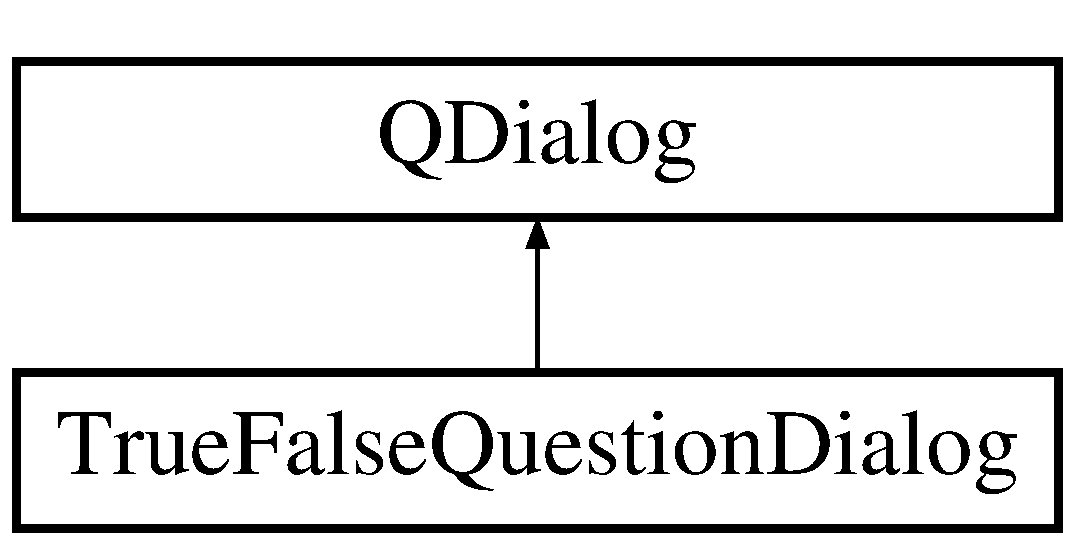
\includegraphics[height=2.000000cm]{class_true_false_question_dialog}
\end{center}
\end{figure}
\subsection*{Public Member Functions}
\begin{DoxyCompactItemize}
\item 
\mbox{\hyperlink{class_true_false_question_dialog_a850bdf7d69a11803b8d15aca1cb824d2}{True\+False\+Question\+Dialog}} (Q\+Widget $\ast$parent=nullptr)
\begin{DoxyCompactList}\small\item\em Fragen\+Dialog. \end{DoxyCompactList}\item 
\mbox{\hyperlink{class_true_false_question_dialog_a13880ffef389859e745013274e68db2f}{$\sim$\+True\+False\+Question\+Dialog}} ()
\item 
void \mbox{\hyperlink{class_true_false_question_dialog_afaebb5ffe9454a723353562edbbfc892}{text\+Random}} (Q\+String \mbox{\hyperlink{class_true_false_question_dialog_a9793a0edd3a9068536a482d1b136785c}{frage}})
\end{DoxyCompactItemize}
\subsection*{Private Slots}
\begin{DoxyCompactItemize}
\item 
void \mbox{\hyperlink{class_true_false_question_dialog_a019068d63e7841958129f4e03f363a65}{on\+\_\+push\+Button\+\_\+\+Ja\+\_\+clicked}} ()
\begin{DoxyCompactList}\small\item\em on\+\_\+push\+Button\+\_\+\+Ja\+\_\+clicked show a feedback if the answer was true or false \end{DoxyCompactList}\item 
void \mbox{\hyperlink{class_true_false_question_dialog_a54e57d5125256a5ea7c7ee58bbba4a10}{on\+\_\+push\+Button\+\_\+\+Next\+\_\+clicked}} ()
\begin{DoxyCompactList}\small\item\em on\+\_\+push\+Button\+\_\+\+Next\+\_\+clicked show the next question \end{DoxyCompactList}\item 
void \mbox{\hyperlink{class_true_false_question_dialog_a3574e49580704a1f20e343b471ca43af}{on\+\_\+push\+Button\+\_\+\+Nein\+\_\+clicked}} ()
\begin{DoxyCompactList}\small\item\em on\+\_\+push\+Button\+\_\+\+Nein\+\_\+clicked show a feedback if the answer was true or false \end{DoxyCompactList}\end{DoxyCompactItemize}
\subsection*{Private Attributes}
\begin{DoxyCompactItemize}
\item 
Ui\+::\+Fragen\+Dialog $\ast$ \mbox{\hyperlink{class_true_false_question_dialog_a2432171c1d7d2f3a798389d9a4d464fc}{ui}}
\item 
Q\+String \mbox{\hyperlink{class_true_false_question_dialog_a9793a0edd3a9068536a482d1b136785c}{frage}} \mbox{[}25\mbox{]}
\begin{DoxyCompactList}\small\item\em frage store the questiones that will be showed to the user \end{DoxyCompactList}\item 
int \mbox{\hyperlink{class_true_false_question_dialog_a8718800a2ddcab39408d0143e2906685}{index}}
\begin{DoxyCompactList}\small\item\em indx save the index of the current showed question \end{DoxyCompactList}\end{DoxyCompactItemize}


\subsection{Detailed Description}
The True\+Falsequestion class show a dialog with a true/false questions to the user. 

\begin{DoxyAuthor}{Author}
Mohamed 
\end{DoxyAuthor}
\begin{DoxyDate}{Date}
22.\+01.\+2019 
\end{DoxyDate}
\begin{DoxyVersion}{Version}
0.\+1 
\end{DoxyVersion}


Definition at line 18 of file truefalsequestiondialog.\+h.



\subsection{Constructor \& Destructor Documentation}
\mbox{\Hypertarget{class_true_false_question_dialog_a850bdf7d69a11803b8d15aca1cb824d2}\label{class_true_false_question_dialog_a850bdf7d69a11803b8d15aca1cb824d2}} 
\index{True\+False\+Question\+Dialog@{True\+False\+Question\+Dialog}!True\+False\+Question\+Dialog@{True\+False\+Question\+Dialog}}
\index{True\+False\+Question\+Dialog@{True\+False\+Question\+Dialog}!True\+False\+Question\+Dialog@{True\+False\+Question\+Dialog}}
\subsubsection{\texorpdfstring{True\+False\+Question\+Dialog()}{TrueFalseQuestionDialog()}}
{\footnotesize\ttfamily True\+False\+Question\+Dialog\+::\+True\+False\+Question\+Dialog (\begin{DoxyParamCaption}\item[{Q\+Widget $\ast$}]{parent = {\ttfamily nullptr} }\end{DoxyParamCaption})\hspace{0.3cm}{\ttfamily [explicit]}}



Fragen\+Dialog. 


\begin{DoxyParams}{Parameters}
{\em parent} & \\
\hline
\end{DoxyParams}


Definition at line 4 of file truefalsequestion\+Dialog.\+cpp.

\mbox{\Hypertarget{class_true_false_question_dialog_a13880ffef389859e745013274e68db2f}\label{class_true_false_question_dialog_a13880ffef389859e745013274e68db2f}} 
\index{True\+False\+Question\+Dialog@{True\+False\+Question\+Dialog}!````~True\+False\+Question\+Dialog@{$\sim$\+True\+False\+Question\+Dialog}}
\index{````~True\+False\+Question\+Dialog@{$\sim$\+True\+False\+Question\+Dialog}!True\+False\+Question\+Dialog@{True\+False\+Question\+Dialog}}
\subsubsection{\texorpdfstring{$\sim$\+True\+False\+Question\+Dialog()}{~TrueFalseQuestionDialog()}}
{\footnotesize\ttfamily True\+False\+Question\+Dialog\+::$\sim$\+True\+False\+Question\+Dialog (\begin{DoxyParamCaption}{ }\end{DoxyParamCaption})}



Definition at line 12 of file truefalsequestion\+Dialog.\+cpp.



\subsection{Member Function Documentation}
\mbox{\Hypertarget{class_true_false_question_dialog_a019068d63e7841958129f4e03f363a65}\label{class_true_false_question_dialog_a019068d63e7841958129f4e03f363a65}} 
\index{True\+False\+Question\+Dialog@{True\+False\+Question\+Dialog}!on\+\_\+push\+Button\+\_\+\+Ja\+\_\+clicked@{on\+\_\+push\+Button\+\_\+\+Ja\+\_\+clicked}}
\index{on\+\_\+push\+Button\+\_\+\+Ja\+\_\+clicked@{on\+\_\+push\+Button\+\_\+\+Ja\+\_\+clicked}!True\+False\+Question\+Dialog@{True\+False\+Question\+Dialog}}
\subsubsection{\texorpdfstring{on\+\_\+push\+Button\+\_\+\+Ja\+\_\+clicked}{on\_pushButton\_Ja\_clicked}}
{\footnotesize\ttfamily void True\+False\+Question\+Dialog\+::on\+\_\+push\+Button\+\_\+\+Ja\+\_\+clicked (\begin{DoxyParamCaption}{ }\end{DoxyParamCaption})\hspace{0.3cm}{\ttfamily [private]}, {\ttfamily [slot]}}



on\+\_\+push\+Button\+\_\+\+Ja\+\_\+clicked show a feedback if the answer was true or false 



Definition at line 18 of file truefalsequestion\+Dialog.\+cpp.

\mbox{\Hypertarget{class_true_false_question_dialog_a3574e49580704a1f20e343b471ca43af}\label{class_true_false_question_dialog_a3574e49580704a1f20e343b471ca43af}} 
\index{True\+False\+Question\+Dialog@{True\+False\+Question\+Dialog}!on\+\_\+push\+Button\+\_\+\+Nein\+\_\+clicked@{on\+\_\+push\+Button\+\_\+\+Nein\+\_\+clicked}}
\index{on\+\_\+push\+Button\+\_\+\+Nein\+\_\+clicked@{on\+\_\+push\+Button\+\_\+\+Nein\+\_\+clicked}!True\+False\+Question\+Dialog@{True\+False\+Question\+Dialog}}
\subsubsection{\texorpdfstring{on\+\_\+push\+Button\+\_\+\+Nein\+\_\+clicked}{on\_pushButton\_Nein\_clicked}}
{\footnotesize\ttfamily void True\+False\+Question\+Dialog\+::on\+\_\+push\+Button\+\_\+\+Nein\+\_\+clicked (\begin{DoxyParamCaption}{ }\end{DoxyParamCaption})\hspace{0.3cm}{\ttfamily [private]}, {\ttfamily [slot]}}



on\+\_\+push\+Button\+\_\+\+Nein\+\_\+clicked show a feedback if the answer was true or false 



Definition at line 58 of file truefalsequestion\+Dialog.\+cpp.

\mbox{\Hypertarget{class_true_false_question_dialog_a54e57d5125256a5ea7c7ee58bbba4a10}\label{class_true_false_question_dialog_a54e57d5125256a5ea7c7ee58bbba4a10}} 
\index{True\+False\+Question\+Dialog@{True\+False\+Question\+Dialog}!on\+\_\+push\+Button\+\_\+\+Next\+\_\+clicked@{on\+\_\+push\+Button\+\_\+\+Next\+\_\+clicked}}
\index{on\+\_\+push\+Button\+\_\+\+Next\+\_\+clicked@{on\+\_\+push\+Button\+\_\+\+Next\+\_\+clicked}!True\+False\+Question\+Dialog@{True\+False\+Question\+Dialog}}
\subsubsection{\texorpdfstring{on\+\_\+push\+Button\+\_\+\+Next\+\_\+clicked}{on\_pushButton\_Next\_clicked}}
{\footnotesize\ttfamily void True\+False\+Question\+Dialog\+::on\+\_\+push\+Button\+\_\+\+Next\+\_\+clicked (\begin{DoxyParamCaption}{ }\end{DoxyParamCaption})\hspace{0.3cm}{\ttfamily [private]}, {\ttfamily [slot]}}



on\+\_\+push\+Button\+\_\+\+Next\+\_\+clicked show the next question 



Definition at line 30 of file truefalsequestion\+Dialog.\+cpp.

\mbox{\Hypertarget{class_true_false_question_dialog_afaebb5ffe9454a723353562edbbfc892}\label{class_true_false_question_dialog_afaebb5ffe9454a723353562edbbfc892}} 
\index{True\+False\+Question\+Dialog@{True\+False\+Question\+Dialog}!text\+Random@{text\+Random}}
\index{text\+Random@{text\+Random}!True\+False\+Question\+Dialog@{True\+False\+Question\+Dialog}}
\subsubsection{\texorpdfstring{text\+Random()}{textRandom()}}
{\footnotesize\ttfamily void True\+False\+Question\+Dialog\+::text\+Random (\begin{DoxyParamCaption}\item[{Q\+String}]{frage }\end{DoxyParamCaption})}



\subsection{Member Data Documentation}
\mbox{\Hypertarget{class_true_false_question_dialog_a9793a0edd3a9068536a482d1b136785c}\label{class_true_false_question_dialog_a9793a0edd3a9068536a482d1b136785c}} 
\index{True\+False\+Question\+Dialog@{True\+False\+Question\+Dialog}!frage@{frage}}
\index{frage@{frage}!True\+False\+Question\+Dialog@{True\+False\+Question\+Dialog}}
\subsubsection{\texorpdfstring{frage}{frage}}
{\footnotesize\ttfamily Q\+String True\+False\+Question\+Dialog\+::frage\mbox{[}25\mbox{]}\hspace{0.3cm}{\ttfamily [private]}}



frage store the questiones that will be showed to the user 



Definition at line 56 of file truefalsequestiondialog.\+h.

\mbox{\Hypertarget{class_true_false_question_dialog_a8718800a2ddcab39408d0143e2906685}\label{class_true_false_question_dialog_a8718800a2ddcab39408d0143e2906685}} 
\index{True\+False\+Question\+Dialog@{True\+False\+Question\+Dialog}!index@{index}}
\index{index@{index}!True\+False\+Question\+Dialog@{True\+False\+Question\+Dialog}}
\subsubsection{\texorpdfstring{index}{index}}
{\footnotesize\ttfamily int True\+False\+Question\+Dialog\+::index\hspace{0.3cm}{\ttfamily [private]}}



indx save the index of the current showed question 



Definition at line 61 of file truefalsequestiondialog.\+h.

\mbox{\Hypertarget{class_true_false_question_dialog_a2432171c1d7d2f3a798389d9a4d464fc}\label{class_true_false_question_dialog_a2432171c1d7d2f3a798389d9a4d464fc}} 
\index{True\+False\+Question\+Dialog@{True\+False\+Question\+Dialog}!ui@{ui}}
\index{ui@{ui}!True\+False\+Question\+Dialog@{True\+False\+Question\+Dialog}}
\subsubsection{\texorpdfstring{ui}{ui}}
{\footnotesize\ttfamily Ui\+::\+Fragen\+Dialog$\ast$ True\+False\+Question\+Dialog\+::ui\hspace{0.3cm}{\ttfamily [private]}}



Definition at line 51 of file truefalsequestiondialog.\+h.



The documentation for this class was generated from the following files\+:\begin{DoxyCompactItemize}
\item 
\mbox{\hyperlink{truefalsequestiondialog_8h}{truefalsequestiondialog.\+h}}\item 
\mbox{\hyperlink{truefalsequestion_dialog_8cpp}{truefalsequestion\+Dialog.\+cpp}}\end{DoxyCompactItemize}

\chapter{File Documentation}
\hypertarget{algebraicprocesses_8cpp}{}\section{algebraicprocesses.\+cpp File Reference}
\label{algebraicprocesses_8cpp}\index{algebraicprocesses.\+cpp@{algebraicprocesses.\+cpp}}
{\ttfamily \#include \char`\"{}algebraicprocesses.\+h\char`\"{}}\newline

\hypertarget{algebraicprocesses_8h}{}\section{algebraicprocesses.\+h File Reference}
\label{algebraicprocesses_8h}\index{algebraicprocesses.\+h@{algebraicprocesses.\+h}}
{\ttfamily \#include \char`\"{}app.\+h\char`\"{}}\newline
{\ttfamily \#include \char`\"{}appstate.\+h\char`\"{}}\newline
{\ttfamily \#include \char`\"{}math.\+h\char`\"{}}\newline
\subsection*{Classes}
\begin{DoxyCompactItemize}
\item 
class \mbox{\hyperlink{class_algebraic_processes}{Algebraic\+Processes}}
\end{DoxyCompactItemize}

\hypertarget{app_8cpp}{}\section{app.\+cpp File Reference}
\label{app_8cpp}\index{app.\+cpp@{app.\+cpp}}
{\ttfamily \#include \char`\"{}app.\+h\char`\"{}}\newline
{\ttfamily \#include $<$iostream$>$}\newline
\subsection*{Namespaces}
\begin{DoxyCompactItemize}
\item 
 \mbox{\hyperlink{namespaceapp}{app}}
\end{DoxyCompactItemize}

\hypertarget{app_8h}{}\section{app.\+h File Reference}
\label{app_8h}\index{app.\+h@{app.\+h}}
{\ttfamily \#include \char`\"{}appstate.\+h\char`\"{}}\newline
{\ttfamily \#include \char`\"{}scene.\+h\char`\"{}}\newline
\subsection*{Classes}
\begin{DoxyCompactItemize}
\item 
class \mbox{\hyperlink{classapp_1_1_app}{app\+::\+App}}
\begin{DoxyCompactList}\small\item\em The \mbox{\hyperlink{classapp_1_1_app}{App}} class it is a basic Point for drawing Programm. \end{DoxyCompactList}\end{DoxyCompactItemize}
\subsection*{Namespaces}
\begin{DoxyCompactItemize}
\item 
 \mbox{\hyperlink{namespaceapp}{app}}
\end{DoxyCompactItemize}

\hypertarget{appstate_8cpp}{}\section{appstate.\+cpp File Reference}
\label{appstate_8cpp}\index{appstate.\+cpp@{appstate.\+cpp}}
{\ttfamily \#include \char`\"{}appstate.\+h\char`\"{}}\newline
{\ttfamily \#include $<$Q\+Debug$>$}\newline
\subsection*{Namespaces}
\begin{DoxyCompactItemize}
\item 
 \mbox{\hyperlink{namespaceapp}{app}}
\end{DoxyCompactItemize}

\hypertarget{appstate_8h}{}\section{appstate.\+h File Reference}
\label{appstate_8h}\index{appstate.\+h@{appstate.\+h}}
{\ttfamily \#include $<$Q\+Color$>$}\newline
{\ttfamily \#include \char`\"{}Q\+Point\char`\"{}}\newline
{\ttfamily \#include $<$Q\+Abstract\+Graphics\+Shape\+Item$>$}\newline
\subsection*{Classes}
\begin{DoxyCompactItemize}
\item 
class \mbox{\hyperlink{classapp_1_1_app_state}{app\+::\+App\+State}}
\begin{DoxyCompactList}\small\item\em This Class Stores the state of the application, for Examble the current tool and it Use default values for all member variables. \end{DoxyCompactList}\end{DoxyCompactItemize}
\subsection*{Namespaces}
\begin{DoxyCompactItemize}
\item 
 \mbox{\hyperlink{namespaceapp}{app}}
\end{DoxyCompactItemize}

\hypertarget{_circle_dialog_8cpp}{}\section{Circle\+Dialog.\+cpp File Reference}
\label{_circle_dialog_8cpp}\index{Circle\+Dialog.\+cpp@{Circle\+Dialog.\+cpp}}
{\ttfamily \#include \char`\"{}circledialog.\+h\char`\"{}}\newline
{\ttfamily \#include \char`\"{}ui\+\_\+rechnendialog.\+h\char`\"{}}\newline
{\ttfamily \#include \char`\"{}math.\+h\char`\"{}}\newline

\hypertarget{circledialog_8h}{}\section{circledialog.\+h File Reference}
\label{circledialog_8h}\index{circledialog.\+h@{circledialog.\+h}}
{\ttfamily \#include $<$Q\+Dialog$>$}\newline
{\ttfamily \#include \char`\"{}Qt\+Core/qmath.\+h\char`\"{}}\newline
\subsection*{Classes}
\begin{DoxyCompactItemize}
\item 
class \mbox{\hyperlink{class_circle_dialog}{Circle\+Dialog}}
\begin{DoxyCompactList}\small\item\em this Dialog show The Component to calculate a Area or Circumfernce from Circle using Radius And vice versa. \end{DoxyCompactList}\end{DoxyCompactItemize}
\subsection*{Namespaces}
\begin{DoxyCompactItemize}
\item 
 \mbox{\hyperlink{namespace_ui}{Ui}}
\end{DoxyCompactItemize}

\hypertarget{ja__nein__fragen_8cpp}{}\section{ja\+\_\+nein\+\_\+fragen.\+cpp File Reference}
\label{ja__nein__fragen_8cpp}\index{ja\+\_\+nein\+\_\+fragen.\+cpp@{ja\+\_\+nein\+\_\+fragen.\+cpp}}
{\ttfamily \#include \char`\"{}ja\+\_\+nein\+\_\+fragen.\+h\char`\"{}}\newline
{\ttfamily \#include \char`\"{}ui\+\_\+ja\+\_\+nein\+\_\+fragen.\+h\char`\"{}}\newline

\hypertarget{ja__nein__fragen_8h}{}\section{ja\+\_\+nein\+\_\+fragen.\+h File Reference}
\label{ja__nein__fragen_8h}\index{ja\+\_\+nein\+\_\+fragen.\+h@{ja\+\_\+nein\+\_\+fragen.\+h}}
{\ttfamily \#include $<$Q\+Main\+Window$>$}\newline
\subsection*{Classes}
\begin{DoxyCompactItemize}
\item 
class \mbox{\hyperlink{class_ja___nein___fragen}{Ja\+\_\+\+Nein\+\_\+\+Fragen}}
\end{DoxyCompactItemize}
\subsection*{Namespaces}
\begin{DoxyCompactItemize}
\item 
 \mbox{\hyperlink{namespace_ui}{Ui}}
\end{DoxyCompactItemize}

\hypertarget{main_8cpp}{}\section{main.\+cpp File Reference}
\label{main_8cpp}\index{main.\+cpp@{main.\+cpp}}
{\ttfamily \#include \char`\"{}mainwindow.\+h\char`\"{}}\newline
{\ttfamily \#include $<$Q\+Application$>$}\newline
\subsection*{Functions}
\begin{DoxyCompactItemize}
\item 
int \mbox{\hyperlink{main_8cpp_a0ddf1224851353fc92bfbff6f499fa97}{main}} (int argc, char $\ast$argv\mbox{[}$\,$\mbox{]})
\end{DoxyCompactItemize}


\subsection{Function Documentation}
\mbox{\Hypertarget{main_8cpp_a0ddf1224851353fc92bfbff6f499fa97}\label{main_8cpp_a0ddf1224851353fc92bfbff6f499fa97}} 
\index{main.\+cpp@{main.\+cpp}!main@{main}}
\index{main@{main}!main.\+cpp@{main.\+cpp}}
\subsubsection{\texorpdfstring{main()}{main()}}
{\footnotesize\ttfamily int main (\begin{DoxyParamCaption}\item[{int}]{argc,  }\item[{char $\ast$}]{argv\mbox{[}$\,$\mbox{]} }\end{DoxyParamCaption})}



Definition at line 4 of file main.\+cpp.


\hypertarget{mainwindow_8cpp}{}\section{mainwindow.\+cpp File Reference}
\label{mainwindow_8cpp}\index{mainwindow.\+cpp@{mainwindow.\+cpp}}
{\ttfamily \#include \char`\"{}mainwindow.\+h\char`\"{}}\newline
{\ttfamily \#include \char`\"{}ui\+\_\+mainwindow.\+h\char`\"{}}\newline
{\ttfamily \#include \char`\"{}Qt\+Core\char`\"{}}\newline
{\ttfamily \#include \char`\"{}Qt\+Gui\char`\"{}}\newline
{\ttfamily \#include \char`\"{}Q\+Message\+Box\char`\"{}}\newline
{\ttfamily \#include \char`\"{}circledialog.\+h\char`\"{}}\newline
{\ttfamily \#include \char`\"{}truefalsequestiondialog.\+h\char`\"{}}\newline

\hypertarget{mainwindow_8h}{}\section{mainwindow.\+h File Reference}
\label{mainwindow_8h}\index{mainwindow.\+h@{mainwindow.\+h}}
{\ttfamily \#include $<$Q\+Main\+Window$>$}\newline
{\ttfamily \#include $<$app.\+h$>$}\newline
{\ttfamily \#include $<$appstate.\+h$>$}\newline
{\ttfamily \#include \char`\"{}Q\+Debug\char`\"{}}\newline
{\ttfamily \#include \char`\"{}rectangledialog.\+h\char`\"{}}\newline
{\ttfamily \#include \char`\"{}squaredialog.\+h\char`\"{}}\newline
{\ttfamily \#include \char`\"{}circledialog.\+h\char`\"{}}\newline
\subsection*{Classes}
\begin{DoxyCompactItemize}
\item 
class \mbox{\hyperlink{class_main_window}{Main\+Window}}
\end{DoxyCompactItemize}
\subsection*{Namespaces}
\begin{DoxyCompactItemize}
\item 
 \mbox{\hyperlink{namespace_ui}{Ui}}
\end{DoxyCompactItemize}

\hypertarget{rectangledialog_8cpp}{}\section{rectangledialog.\+cpp File Reference}
\label{rectangledialog_8cpp}\index{rectangledialog.\+cpp@{rectangledialog.\+cpp}}
{\ttfamily \#include \char`\"{}rectangledialog.\+h\char`\"{}}\newline
{\ttfamily \#include \char`\"{}ui\+\_\+rectangledialog.\+h\char`\"{}}\newline

\hypertarget{rectangledialog_8h}{}\section{rectangledialog.\+h File Reference}
\label{rectangledialog_8h}\index{rectangledialog.\+h@{rectangledialog.\+h}}
{\ttfamily \#include $<$Q\+Dialog$>$}\newline
\subsection*{Classes}
\begin{DoxyCompactItemize}
\item 
class \mbox{\hyperlink{class_rectangle_dialog}{Rectangle\+Dialog}}
\begin{DoxyCompactList}\small\item\em The \mbox{\hyperlink{class_rectangle_dialog}{Rectangle\+Dialog}} class show a dialog with options to calculate the area, circumference and side of rectangle. \end{DoxyCompactList}\end{DoxyCompactItemize}
\subsection*{Namespaces}
\begin{DoxyCompactItemize}
\item 
 \mbox{\hyperlink{namespace_ui}{Ui}}
\end{DoxyCompactItemize}

\hypertarget{scene_8cpp}{}\section{scene.\+cpp File Reference}
\label{scene_8cpp}\index{scene.\+cpp@{scene.\+cpp}}
{\ttfamily \#include \char`\"{}scene.\+h\char`\"{}}\newline

\hypertarget{scene_8h}{}\section{scene.\+h File Reference}
\label{scene_8h}\index{scene.\+h@{scene.\+h}}
{\ttfamily \#include $<$Q\+Graphics\+Scene$>$}\newline
{\ttfamily \#include \char`\"{}Q\+Mouse\+Event\char`\"{}}\newline
\subsection*{Classes}
\begin{DoxyCompactItemize}
\item 
class \mbox{\hyperlink{class_scene}{Scene}}
\end{DoxyCompactItemize}

\hypertarget{squaredialog_8cpp}{}\section{squaredialog.\+cpp File Reference}
\label{squaredialog_8cpp}\index{squaredialog.\+cpp@{squaredialog.\+cpp}}
{\ttfamily \#include \char`\"{}squaredialog.\+h\char`\"{}}\newline
{\ttfamily \#include \char`\"{}ui\+\_\+squaredialog.\+h\char`\"{}}\newline
{\ttfamily \#include \char`\"{}math.\+h\char`\"{}}\newline

\hypertarget{squaredialog_8h}{}\section{squaredialog.\+h File Reference}
\label{squaredialog_8h}\index{squaredialog.\+h@{squaredialog.\+h}}
{\ttfamily \#include \char`\"{}Qt\+Core/qmath.\+h\char`\"{}}\newline
{\ttfamily \#include $<$Q\+Dialog$>$}\newline
\subsection*{Classes}
\begin{DoxyCompactItemize}
\item 
class \mbox{\hyperlink{class_square_dialog}{Square\+Dialog}}
\begin{DoxyCompactList}\small\item\em The \mbox{\hyperlink{class_square_dialog}{Square\+Dialog}} class show a dialog with options to calculate the Area, circumference und side of the square. \end{DoxyCompactList}\end{DoxyCompactItemize}
\subsection*{Namespaces}
\begin{DoxyCompactItemize}
\item 
 \mbox{\hyperlink{namespace_ui}{Ui}}
\end{DoxyCompactItemize}

\hypertarget{truefalsequestion_dialog_8cpp}{}\section{truefalsequestion\+Dialog.\+cpp File Reference}
\label{truefalsequestion_dialog_8cpp}\index{truefalsequestion\+Dialog.\+cpp@{truefalsequestion\+Dialog.\+cpp}}
{\ttfamily \#include \char`\"{}truefalsequestiondialog.\+h\char`\"{}}\newline
{\ttfamily \#include \char`\"{}ui\+\_\+fragendialog.\+h\char`\"{}}\newline

\hypertarget{truefalsequestiondialog_8h}{}\section{truefalsequestiondialog.\+h File Reference}
\label{truefalsequestiondialog_8h}\index{truefalsequestiondialog.\+h@{truefalsequestiondialog.\+h}}
{\ttfamily \#include $<$Q\+Dialog$>$}\newline
{\ttfamily \#include \char`\"{}Q\+Message\+Box\char`\"{}}\newline
\subsection*{Classes}
\begin{DoxyCompactItemize}
\item 
class \mbox{\hyperlink{class_true_false_question_dialog}{True\+False\+Question\+Dialog}}
\begin{DoxyCompactList}\small\item\em The True\+Falsequestion class show a dialog with a true/false questions to the user. \end{DoxyCompactList}\end{DoxyCompactItemize}
\subsection*{Namespaces}
\begin{DoxyCompactItemize}
\item 
 \mbox{\hyperlink{namespace_ui}{Ui}}
\end{DoxyCompactItemize}

%--- End generated contents ---

% Index
\backmatter
\newpage
\phantomsection
\clearemptydoublepage
\addcontentsline{toc}{chapter}{Index}
\printindex

\end{document}
